% ============================================================
%  NIS2 Management Training — PDF Book
%  Compile with: pdflatex nis2-management-training.tex
%  Requires: xelatex or pdflatex (recommended: pdflatex twice)
%  Packages: geometry, tcolorbox, tikz, xcolor, enumitem,
%            hyperref, booktabs, multicol, mdframed, fontenc
% ============================================================

\documentclass[11pt,a4paper,twoside]{book}

%  Encoding & Fonts 
\usepackage[T1]{fontenc}
\usepackage[utf8]{inputenc}
\usepackage{lmodern}
\usepackage{microtype}

%  Math symbols (for \checkmark, etc.) 
\usepackage{amssymb}
\usepackage{amsmath}

%  Euro symbol 
\usepackage{eurosym}

%  Layout 
\usepackage[
  top=25mm, bottom=25mm,
  inner=28mm, outer=20mm,
  headheight=14pt
]{geometry}
\usepackage{fancyhdr}
\usepackage{emptypage}

%  Colors 
\usepackage{xcolor}
\definecolor{nisd2blue}{HTML}{284b63}
\definecolor{nisd2mid}{HTML}{3a6b8a}
\definecolor{nisd2light}{HTML}{d0e4f0}
\definecolor{nisd2accent}{HTML}{e8824a}
\definecolor{warningred}{HTML}{c0392b}
\definecolor{successgreen}{HTML}{27ae60}
\definecolor{quizgray}{HTML}{f4f6f8}
\definecolor{correctgreen}{HTML}{d5f0dc}
\definecolor{keybox}{HTML}{fef9ec}
\definecolor{keyboxborder}{HTML}{f0c040}
\definecolor{actionbox}{HTML}{eaf4fb}
\definecolor{actionborder}{HTML}{3a6b8a}

%  Graphics & Diagrams 
\usepackage{tikz}
\usetikzlibrary{shapes.geometric, arrows.meta, positioning, fit, backgrounds, calc}
\usepackage{graphicx}

%  Boxes 
\usepackage[most]{tcolorbox}
\tcbuselibrary{skins, breakable}

%  Lists 
\usepackage{enumitem}
\setlist[itemize]{leftmargin=*, noitemsep, topsep=2pt}
\setlist[enumerate]{leftmargin=*, noitemsep, topsep=2pt}

%  Tables 
\usepackage{booktabs}
\usepackage{tabularx}
\usepackage{array}
\usepackage{multirow}

%  Multi-column 
\usepackage{multicol}

%  Chapter/Section Styling 
\usepackage{titlesec}

\titleformat{\chapter}[display]
  {\normalfont\huge\bfseries\color{nisd2blue}}
  {\chaptertitlename\ \thechapter}{12pt}{\Huge}
\titleformat{\section}
  {\normalfont\Large\bfseries\color{nisd2blue}}
  {\thesection}{1em}{}
\titleformat{\subsection}
  {\normalfont\large\bfseries\color{nisd2mid}}
  {\thesubsection}{1em}{}

%  Headers & Footers 
\pagestyle{fancy}
\fancyhf{}
\fancyhead[LE]{\small\nouppercase{\textcolor{nisd2blue}{\leftmark}}}
\fancyhead[RO]{\small\nouppercase{\textcolor{nisd2blue}{\rightmark}}}
\fancyfoot[LE,RO]{\small\thepage}
\fancyfoot[CE,CO]{\small\textcolor{nisd2mid}{NIS2 Management Training}}
\renewcommand{\headrulewidth}{0.4pt}
\renewcommand{\headrule}{\hbox to\headwidth{\color{nisd2light}\leaders\hrule height \headrulewidth\hfill}}

%  Hyperlinks 
\usepackage{hyperref}
\hypersetup{
  colorlinks=true,
  linkcolor=nisd2blue,
  urlcolor=nisd2mid,
  citecolor=nisd2mid,
  pdftitle={NIS2 Management Training},
  pdfauthor={NISD2},
  pdfsubject={NIS2 Directive — Management Body Training},
  bookmarksnumbered=true
}

% ============================================================
%  Custom Environments
% ============================================================

% Key Takeaways box
\newtcolorbox{keytakeaways}{
  enhanced, breakable,
  colback=keybox,
  colframe=keyboxborder,
  fonttitle=\bfseries\color{nisd2blue},
  title={Key Takeaways},
  left=6pt, right=6pt, top=4pt, bottom=4pt,
  arc=3pt
}

% Action Item box
\newtcolorbox{actionbox}{
  enhanced, breakable,
  colback=actionbox,
  colframe=actionborder,
  fonttitle=\bfseries\color{nisd2blue},
  title={Ask Your Team},
  left=6pt, right=6pt, top=4pt, bottom=4pt,
  arc=3pt
}

% Warning / Liability box
\newtcolorbox{warningbox}{
  enhanced, breakable,
  colback=white,
  colframe=warningred,
  fonttitle=\bfseries\color{warningred},
  title={Personal Liability Note},
  left=6pt, right=6pt, top=4pt, bottom=4pt,
  arc=3pt
}

% Quiz container
\newtcolorbox{quizbox}{
  enhanced, breakable,
  colback=quizgray,
  colframe=nisd2mid,
  fonttitle=\bfseries\color{white},
  coltitle=white,
  attach boxed title to top left={yshift=-2mm, xshift=4mm},
  boxed title style={colback=nisd2mid, arc=2pt},
  title={Quiz},
  left=6pt, right=6pt, top=8pt, bottom=4pt,
  arc=3pt
}

% Correct answer highlight
\newtcolorbox{correctanswer}{
  enhanced,
  colback=correctgreen,
  colframe=successgreen,
  left=4pt, right=4pt, top=2pt, bottom=2pt,
  arc=2pt, boxrule=0.5pt
}

% Definition box
\newtcolorbox{definitionbox}[1]{
  enhanced,
  colback=nisd2light!40,
  colframe=nisd2mid,
  fonttitle=\bfseries\small\color{nisd2blue},
  title={#1},
  left=5pt, right=5pt, top=3pt, bottom=3pt,
  arc=2pt
}

% Case study box
\newtcolorbox{casestudy}[1]{
  enhanced, breakable,
  colback=white,
  colframe=nisd2accent,
  fonttitle=\bfseries\color{nisd2accent},
  title={Case Study: #1},
  left=6pt, right=6pt, top=4pt, bottom=4pt,
  arc=3pt
}

% Module intro box
\newtcolorbox{moduleintro}{
  enhanced,
  colback=nisd2blue,
  colframe=nisd2blue,
  coltext=white,
  left=10pt, right=10pt, top=8pt, bottom=8pt,
  arc=4pt
}

% Lesson number command (colorbox, safe in section headings + TOC)
\newcommand{\lessontag}[1]{%
  \texorpdfstring{%
    \setlength{\fboxsep}{3pt}\colorbox{nisd2blue}{\textcolor{white}{\footnotesize\bfseries #1}}\quad%
  }{Lesson #1\ }%
}

% Quiz question environment
\newcounter{quizq}
\newcommand{\quizquestion}[2]{%
  \stepcounter{quizq}
  \vspace{4pt}
  \noindent\textbf{Q\thequizq.} #1
  \vspace{2pt}
  \begin{enumerate}[label=\Alph*., leftmargin=16pt, noitemsep]
    #2
  \end{enumerate}
}

%  Answer key tracking 
% Write answers to .ans file; appendix reads them back
\newwrite\answerfile
\immediate\openout\answerfile=\jobname.ans

% correct: plain output (no highlight), writes lesson + Q + letter to file
\newcommand{\correct}[1]{%
  #1%
  \immediate\write\answerfile{\string\ansentry{\thesection}{\thequizq}{\Alph{enumi}}}%
}

% ansentry rendering (used in appendix via \input)
\newcommand{\currentanslesson}{}
\newcommand{\ansentry}[3]{%
  \def\thislesson{#1}%
  \ifx\thislesson\currentanslesson\else%
    \medskip\noindent\textbf{\small Lesson #1}\nopagebreak\par%
    \global\def\currentanslesson{#1}%
  \fi%
  \noindent\hspace{1.5em}{\small Q#2:~\textbf{#3}}\par%
}

% Explanation box inside quiz
\newcommand{\quizexplain}[1]{%
  \vspace{2pt}
  \noindent\small\textit{\textcolor{nisd2mid}{#1}}
  \vspace{6pt}
}

% Course version — bump this when publishing a new PDF to public/downloads/
\newcommand{\courseversion}{v1.0.0}

% ============================================================
%  Document
% ============================================================

\begin{document}

%  Title Page 
\begin{titlepage}
  \pagecolor{nisd2blue}
  \color{white}
  \vspace*{2cm}
  \begin{center}
    \begin{tikzpicture}
      \node[circle, fill=white, minimum size=2.8cm] (logo) at (0,0) {
        \textcolor{nisd2blue}{\Large\bfseries NIS2}
      };
    \end{tikzpicture}

    \vspace{1.2cm}
    {\fontsize{36}{42}\selectfont\bfseries NIS2 Management Training}

    \vspace{0.6cm}
    {\Large\bfseries Everything the Directive Requires\\[4pt]
    a Member of the Management Body to Know}

    \vspace{1.2cm}
    \begin{tikzpicture}
      \draw[white, line width=0.5pt] (0,0) -- (10,0);
    \end{tikzpicture}

    \vspace{0.8cm}
    {\large Structured around the BSI's three competence areas\\
    and the ten Article~21 measures}

    \vspace{1.6cm}
    \begin{tikzpicture}
      \foreach \i/\label in {
        0/The Law,
        72/Risk \& the\\10 Measures,
        144/Decision\\Support,
        216/Protection,
        288/Final}{
        \node[circle, fill=white!20, text=white, minimum size=1.8cm,
              font=\small\bfseries, align=center] at (\i:3.2cm) {\label};
      }
      \node[circle, fill=white, text=nisd2blue, minimum size=1.6cm,
            font=\bfseries, align=center] at (0,0) {5\\Modules};
    \end{tikzpicture}

    \vspace{1.6cm}
    {\small\bfseries 47 Lessons\ \ $\bullet$\ \ 4 Hours of Content\ \
    $\bullet$\ \ Quiz After Every Lesson}

    \vspace{0.6cm}
    {\small \courseversion \quad NISD2 — \texttt{www.nisd2.eu}}
  \end{center}
  \pagecolor{white}
  \color{black}
\end{titlepage}

%  Copyright / Disclaimer 
\thispagestyle{empty}
\vspace*{\fill}
\begin{small}
\noindent\textbf{About this book}

This book is a print-ready version of the NIS2 Management Training course available at \texttt{www.nisd2.eu}. It follows the three competence areas required by Article~20(2) of the NIS2 Directive: identifying risks, assessing the measures used to manage them, and understanding how those risks affect the services your company delivers.

\vspace{6pt}
\noindent\textbf{Not legal advice.} This course teaches the EU directive and the concepts behind it. It is not legal advice, and no body in the European Union currently certifies NIS2 trainers or training programmes. This document is training material, not a legal certification.

\vspace{6pt}
\noindent\textbf{German standard.} Throughout this course we reference the German implementatio, the BSIG and the BSI, because Germany's transposition is the strictest in the EU. If you build your compliance to the German standard, you meet or exceed requirements in every other member state.

\vspace{6pt}
\noindent\textbf{Passing score.} Each lesson quiz requires 75\% to pass.

\vspace{6pt}
\noindent\textbf{Licence.} $\copyright$ 2026 Kardashev Catalyst UG (haftungsbeschränkt). This material is licensed under the Creative Commons Attribution 4.0 International License (CC BY 4.0), \texttt{creativecommons.org/licenses/by/4.0/}. You may share, shorten, translate and adapt it, and publish the result under your own name, including commercially. Attribution is the only condition. Chambers of commerce, associations and educational institutions are expressly invited to do so.
\end{small}
\vspace*{\fill}
\newpage

%  Table of Contents 
\tableofcontents
\newpage

% ============================================================
%  PREFACE / FOUNDATION
% ============================================================

\chapter*{About This Course}
\addcontentsline{toc}{chapter}{About This Course}
\markboth{About This Course}{About This Course}

EU law now requires every member of a management body of a covered company to personally undergo cybersecurity training. Not your CISO. Not your head of IT. \textbf{You.} Article~20(2) of the NIS2 Directive, written into national law in every EU country, names the leadership team directly.

\section*{Who this course is for}

If you sit on the leadership team of a company covered by NIS2 as a CEO, managing director, executive board member, COO, CFO, or any role the law calls a ``member of the management body''  this course is for you. The law does not distinguish between the CEO and the rest of the leadership team. Every single member carries the same duty. \textbf{The training obligation is non-delegable.} You cannot send your CISO, your lawyer, or your assistant in your place.

\section*{What this course is}

This is a structured course covering what the NIS2 Directive requires you to know as a member of the leadership team. It follows the three competence areas the law requires:
\begin{itemize}
  \item \textbf{Identifying risks} understanding what threats your company faces
  \item \textbf{Assessing the measures} evaluating whether what your team has put in place actually works
  \item \textbf{Understanding service impact} connecting cybersecurity to your business operations
\end{itemize}

Forty-seven short lessons. Roughly four hours of content and review. After every lesson there is a short quiz. When you complete the course, the platform issues a Certificate of Completion in your name.

\section*{What this course is not}

This course is not legal advice. This course is not a certified qualification. No body in the European Union currently certifies NIS2 trainers or training programmes.

\section*{How to use this book}

Work through each chapter in order. After each lesson, complete the quiz. When a specific requirement lands a signature you have to give, a document you have to personally approve write it down. By the end you will have your own action list.

\begin{keytakeaways}
\begin{enumerate}
\item Article~20(2) of the NIS2 Directive personally requires every member of the management body to undergo cybersecurity training the duty is non-delegable.
  \item No EU member state has established a state-backed certification for NIS2 training; the auditor judges sufficiency based on content covered, time spent, and documentation.
  \item This course covers all three competence areas the law requires.
\end{enumerate}
\end{keytakeaways}

\newpage

% ============================================================
%  CHAPTER 1: THE LAW
% ============================================================

\chapter{The Law}

\begin{moduleintro}
\textbf{Module 1 12 Lessons}

This module covers the legal foundation of NIS2: what the law is, who it applies to, what it requires you personally to do, and what happens if you do not. By the end, you will be able to answer the five foundation questions the BSI expects every covered CEO to answer.
\end{moduleintro}

\bigskip

% === LEGAL ARCHITECTURE DIAGRAM ===

\begin{center}
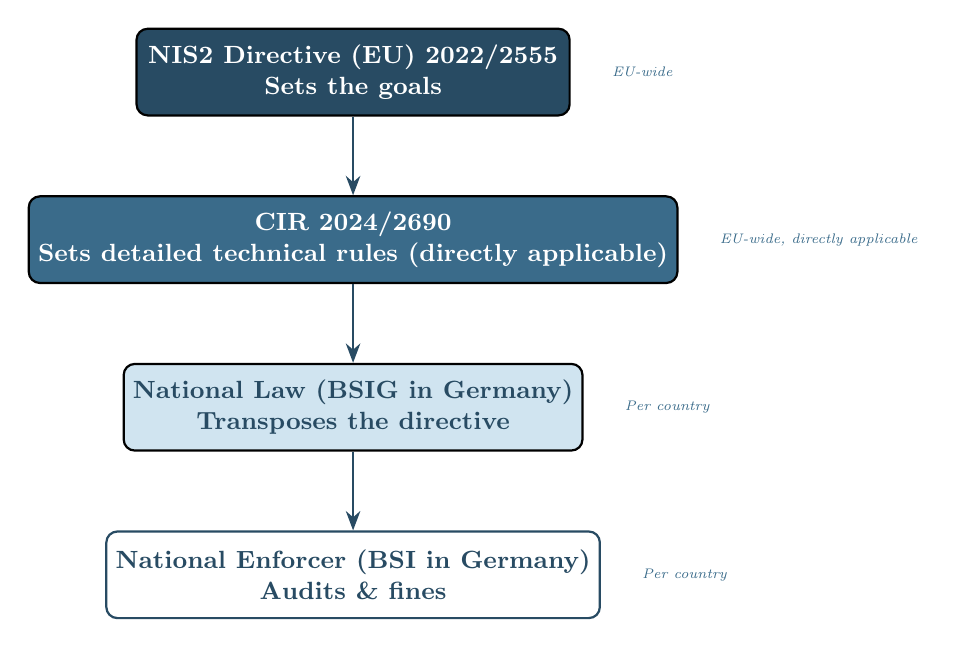
\begin{tikzpicture}[
  node distance=1.0cm,
  box/.style={rectangle, rounded corners=4pt, draw, thick,
    minimum width=5.5cm, minimum height=1.1cm, align=center,
    font=\small\bfseries},
  arrow/.style={-{Stealth[length=7pt]}, thick, color=nisd2blue}
]

\node[box, fill=nisd2blue, text=white] (nis2)
  {NIS2 Directive (EU) 2022/2555\\Sets the goals};

\node[box, fill=nisd2mid, text=white, below=of nis2] (cir)
  {CIR 2024/2690\\Sets detailed technical rules (directly applicable)};

\node[box, fill=nisd2light, text=nisd2blue, below=of cir] (natlaw)
  {National Law (BSIG in Germany)\\Transposes the directive};

\node[box, fill=white, draw=nisd2blue, text=nisd2blue, below=of natlaw] (bsi)
  {National Enforcer (BSI in Germany)\\Audits \& fines};

\draw[arrow] (nis2) -- (cir);
\draw[arrow] (cir) -- (natlaw);
\draw[arrow] (natlaw) -- (bsi);

\node[right=0.4cm of nis2, font=\tiny\itshape, text=nisd2mid] {EU-wide};
\node[right=0.4cm of cir, font=\tiny\itshape, text=nisd2mid] {EU-wide, directly applicable};
\node[right=0.4cm of natlaw, font=\tiny\itshape, text=nisd2mid] {Per country};
\node[right=0.4cm of bsi, font=\tiny\itshape, text=nisd2mid] {Per country};
\end{tikzpicture}
\par\smallskip\noindent{\small\textit{The full legal chain from EU directive to national enforcement.}}
\end{center}

\bigskip

%  LESSON 1.1 
\section{\lessontag{1.1}What NIS2 Is and Why It Exists}

Roughly 160,000 companies across the European Union are now on a list the EU decided is too important to go dark. If your company is on that list, the rules governing your cybersecurity are no longer set by you, they are set by three layers of EU and national law, enforced by a national regulator.

\subsection*{The Directive}

The formal name is Directive (EU) 2022/2555 the \textbf{NIS2 Directive}. Adopted on 14 December 2022, entered into force on 16 January 2023. It replaces NIS1, which was widely seen as inconsistent and weakly enforced, almost no fines were ever issued under NIS1 anywhere in the EU.

NIS2 is a \textbf{directive}, not a regulation. A regulation (like the GDPR) applies directly in every country. A directive tells each country what the result has to be, and each country writes its own national law. The directive is the floor, not the ceiling.

\subsection*{The Implementing Regulation (CIR)}

Commission Implementing Regulation (EU) 2024/2690 is a regulation it applies directly in all 27 member states without transposition. The CIR sets the detailed technical requirements: what counts as a significant incident, what policies you must have, what thresholds trigger mandatory reporting.

\subsection*{The Enforcer}

In Germany: the BSIG (Federal IT Security Act) and the BSI (Federal Office for Information Security). The BSI can audit, require registration, require incident reports, and impose fines up to \textbf{€10 million or 2\% of global turnover}.

\begin{keytakeaways}
\begin{enumerate}
  \item NIS2 is Directive (EU) 2022/2555 one EU-wide cybersecurity law covering roughly 160,000 entities.
  \item Three layers apply: the NIS2 Directive (goals), the CIR 2024/2690 (detailed technical rules, directly applicable), and national law (BSIG in Germany) enforced by the BSI.
  \item The directive creates personal accountability for the management body which is why leadership, not just IT, is addressed directly.
\end{enumerate}
\end{keytakeaways}

\begin{quizbox}
\setcounter{quizq}{0}

\quizquestion{What is the difference between an EU directive and an EU regulation?}{
  \item A directive applies directly; a regulation must be transposed into national law
  \item \correct{A regulation applies directly; a directive must be transposed into national law}
  \item There is no difference; both apply directly
  \item A directive only applies to Essential entities; a regulation applies to all
}
\quizexplain{A regulation (like the GDPR or the CIR) applies directly in every country. A directive tells each country what the result has to be, and each country writes its own national law.}

\quizquestion{What does the CIR (Commission Implementing Regulation 2024/2690) do?}{
  \item It replaces the NIS2 Directive entirely
  \item It sets the goals that each country must achieve
  \item \correct{It sets detailed technical requirements that apply directly in all 27 member states}
  \item It designates the competent authority in each country
}
\quizexplain{The CIR is a regulation that applies directly in all member states, setting detailed technical requirements.}

\quizquestion{What is the full legal chain?}{
  \item CIR sets goals, NIS2 sets rules, national law enforces
  \item \correct{NIS2 Directive sets goals, CIR sets detailed technical rules, national law transposes, national enforcer audits}
  \item National law sets goals, NIS2 Directive sets rules, CIR enforces
  \item GDPR sets goals, NIS2 sets rules, CIR enforces
}
\quizexplain{EU Directive (NIS2) → goals; EU Regulation (CIR) → detailed technical rules; national law → transposes; national enforcer → audits and fines.}

\quizquestion{Why was NIS1 replaced?}{
  \item NIS1 was too strict and costly for companies
  \item NIS1 only applied to digital infrastructure providers
  \item \correct{NIS1 was widely seen as inconsistent and weakly enforced, with almost no fines ever issued}
  \item NIS1 was a regulation that could not be adapted to local laws
}
\quizexplain{Almost no fines were ever issued under NIS1 anywhere in the EU. NIS2 was designed to fix this.}
\end{quizbox}

% , LESSON 1.2 ,
\section{\lessontag{1.2}Who Is in Scope Essential vs Important Entities}

Article~3 of the NIS2 Directive sorts covered companies into two lists.

\begin{center}
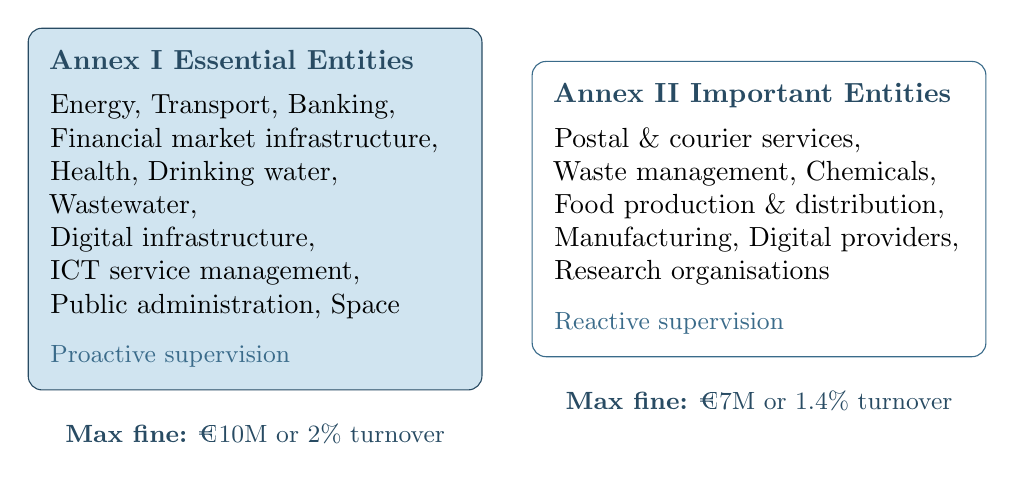
\begin{tikzpicture}
\node[rectangle, rounded corners=5pt, draw=nisd2blue, fill=nisd2light,
      minimum width=5.5cm, minimum height=3.2cm, text width=5.2cm,
      align=flush left, inner sep=8pt] (essential) at (-3.2,0) {
  \textbf{\textcolor{nisd2blue}{Annex I Essential Entities}}\\[4pt]
  Energy, Transport, Banking,\\
  Financial market infrastructure,\\
  Health, Drinking water, Wastewater,\\
  Digital infrastructure,\\
  ICT service management,\\
  Public administration, Space\\[6pt]
  \textcolor{nisd2mid}{\small Proactive supervision}
};
\node[rectangle, rounded corners=5pt, draw=nisd2mid, fill=white,
      minimum width=5.5cm, minimum height=3.2cm, text width=5.2cm,
      align=flush left, inner sep=8pt] (important) at (3.2,0) {
  \textbf{\textcolor{nisd2blue}{Annex II Important Entities}}\\[4pt]
  Postal \& courier services,\\
  Waste management, Chemicals,\\
  Food production \& distribution,\\
  Manufacturing, Digital providers,\\
  Research organisations\\[6pt]
  \textcolor{nisd2mid}{\small Reactive supervision}
};
\node[below=0.3cm of essential, font=\small, text=nisd2blue]
  {\textbf{Max fine:} €10M or 2\% turnover};
\node[below=0.3cm of important, font=\small, text=nisd2blue]
  {\textbf{Max fine:} €7M or 1.4\% turnover};
\end{tikzpicture}
\end{center}

\textbf{Size threshold:} 50+ employees \emph{or} \textgreater €10M annual turnover. Meet either criterion and operate in a listed sector: you are in scope.

\textbf{The key difference:} Essential entities face \emph{proactive} supervision (audited any time, no cause needed). Important entities face \emph{reactive} supervision (audited when triggered). \textbf{The ten measures under Article~21 apply equally to both.}

\begin{keytakeaways}
\begin{enumerate}
  \item NIS2 covers two categories, Essential (Annex I) and Important (Annex II) with a size threshold of 50 employees or €10M turnover for both.
  \item Essential entities face proactive supervision. Important entities face reactive supervision.
  \item The ten measures apply equally to both categories, the difference is enforcement intensity, not compliance scope.
\end{enumerate}
\end{keytakeaways}

\begin{quizbox}
\setcounter{quizq}{0}
\quizquestion{What is the size threshold for most companies to fall in scope of NIS2?}{
  \item 250 or more employees, or €50M in turnover
  \item \correct{50 or more employees, or more than €10M in annual turnover}
  \item 10 or more employees, or more than €1M in annual turnover
  \item 100 or more employees, or more than €25M in annual turnover
}
\quizexplain{The general threshold is 50+ employees or \textgreater €10M turnover in a listed sector.}

\quizquestion{What is the key difference between Essential and Important entities?}{
  \item Essential entities must implement all ten measures; Important entities only implement five
  \item \correct{Essential entities face proactive supervision; Important entities face reactive supervision}
  \item Important entities face higher fines than Essential entities
  \item Essential entities are in Annex II; Important entities are in Annex I
}

\quizquestion{Do Essential and Important entities implement different security measures?}{
  \item Yes, Essential entities have stricter technical requirements
  \item Yes, Important entities have additional reporting duties
  \item \correct{No, both must implement the same ten measures under Article~21}
  \item No measures apply to Important entities
}
\end{quizbox}

%  LESSON 1.3 
\section{\lessontag{1.3}Penalties and the Article 34 Manager Ban}

\begin{center}
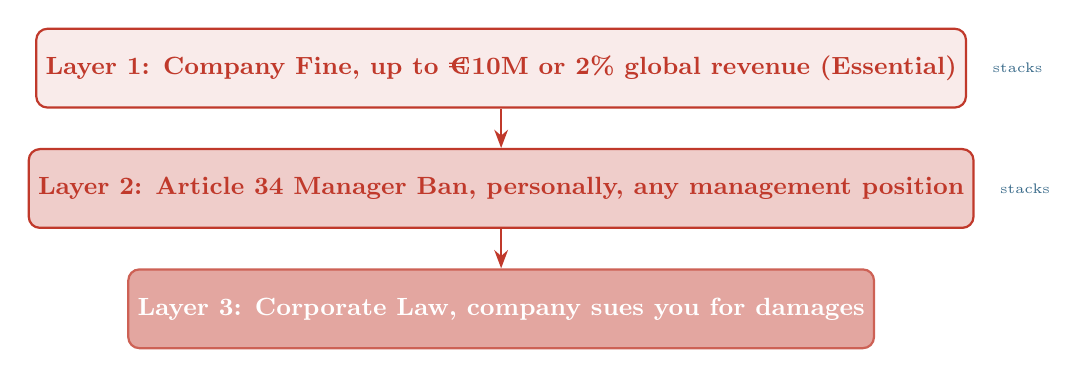
\begin{tikzpicture}[
  layer/.style={rectangle, rounded corners=4pt, draw, thick,
    minimum width=8cm, minimum height=1.0cm, align=center, font=\small\bfseries}
]
\node[layer, fill=warningred!10, draw=warningred] (l1) at (0, 0)
  {\textcolor{warningred}{Layer 1: Company Fine, up to €10M or 2\% global revenue (Essential)}};
\node[layer, fill=warningred!25, draw=warningred, below=0.5cm of l1] (l2)
  {\textcolor{warningred}{Layer 2: Article 34 Manager Ban, personally, any management position}};
\node[layer, fill=warningred!45, draw=warningred!80, below=0.5cm of l2] (l3)
  {\textcolor{white}{Layer 3: Corporate Law, company sues you for damages}};

\draw[-{Stealth}, thick, warningred] (l1.south) -- (l2.north);
\draw[-{Stealth}, thick, warningred] (l2.south) -- (l3.north);

\node[right=0.2cm of l1, font=\tiny, text=nisd2mid] {stacks};
\node[right=0.2cm of l2, font=\tiny, text=nisd2mid] {stacks};
\end{tikzpicture}
\end{center}

Three layers of exposure. \textbf{They stack.} The regulator can fine the company, ban you personally, and the company can sue you for damages, all for the same failure.

Article~20(1) makes this explicit: management bodies ``can be held liable for infringements.''

\begin{warningbox}
Article~34 includes \textbf{interim management restrictions}: a temporary removal from office \emph{while the investigation is still running}. You can be removed before the case is decided.
\end{warningbox}

\begin{keytakeaways}
\begin{enumerate}
  \item The company fine caps at €10M or 2\% global revenue for Essential entities; €7M or 1.4\% for Important. Member states can go higher.
  \item Article~34 gives the regulator the power to ban you, personally, from holding any management position, including an interim removal while proceedings run.
  \item Your national corporate law lets the company sue you personally for damages on top of both the fine and the ban.
\end{enumerate}
\end{keytakeaways}

\begin{quizbox}
\setcounter{quizq}{0}
\quizquestion{What is the maximum fine for Essential entities under NIS2?}{
  \item €7M or 1.4\% of worldwide turnover
  \item \correct{€10M or 2\% of worldwide annual turnover, whichever is higher}
  \item €5M or 1\% of worldwide turnover
  \item €20M or 4\% of worldwide turnover
}
\quizquestion{What does Article~34 allow the regulator to do?}{
  \item Only fine the company
  \item \correct{Ban an individual from holding any management position, including interim removal during investigation}
  \item Shut down the company permanently
  \item Revoke the company's operating licence
}
\quizquestion{How many layers of exposure does the lesson describe?}{
  \item One: the company fine
  \item Two: the company fine and the manager ban
  \item \correct{Three: the company fine, the Article~34 manager ban, and personal civil liability under corporate law}
  \item Four: fine, ban, civil liability, and criminal prosecution
}
\quizquestion{What is the maximum fine cap for Important entities?}{
  \item €10M or 2\% of worldwide turnover
  \item \correct{€7M or 1.4\% of worldwide turnover, whichever is higher}
  \item €5M or 1\% of worldwide turnover
  \item There is no cap for Important entities
}
\end{quizbox}

%  LESSON 1.4 
\section{\lessontag{1.4}The Registration Obligation}

Article~27 of the NIS2 Directive requires covered companies to \textbf{register with the national competent authority within three months} of becoming subject to NIS2.

\begin{definitionbox}{What the registration must include}
Company name, address, sector, contact details \textbf{including a 24/7 incident contact}, the services the company provides, the EU countries where those services are offered, and (for digital infrastructure providers) IP address ranges.
\end{definitionbox}

Late or incorrect registration is sanctioned separately under Article~32, its own violation, independent of any cyber incident. In Germany as of March 2026, roughly \textbf{11,500 of an estimated 29,500} in-scope companies had registered by the deadline.

\begin{keytakeaways}
\begin{enumerate}
  \item Article~27 gives you three months from the day your company becomes covered to register, and must include a 24/7 incident contact.
  \item Missing or incorrect registration is a separate fine, independent of any cyber incident, and is the easiest violation for the regulator to detect.
  \item In Germany, only about 11,500 of an estimated 29,500 in-scope companies had registered by March 2026, the rest are exposed to immediate enforcement.
\end{enumerate}
\end{keytakeaways}

\begin{quizbox}
\setcounter{quizq}{0}
\quizquestion{How long does a company have to register after becoming covered?}{
  \item One month
  \item \correct{Three months}
  \item Six months
  \item One year
}
\quizquestion{Is missing registration a violation even without a cyber incident?}{
  \item No, a violation requires a cyber incident
  \item \correct{Yes, it is a separate violation sanctioned under Article~32, independent of any incident}
  \item Only if the regulator has already audited the company
  \item Only for Essential entities
}
\quizquestion{What specific contact must be included in the NIS2 registration?}{
  \item The CEO's personal mobile number
  \item \correct{A twenty-four-seven incident contact}
  \item The company's general email address
  \item The CISO's LinkedIn profile
}
\end{quizbox}

%  LESSON 1.5 
\section{\lessontag{1.5}Your Duty to Approve and Oversee}

Article~20(1) of the NIS2 Directive: \textit{``the management bodies of essential and important entities approve the cybersecurity risk-management measures taken by those entities in order to comply with Article~21, oversee its implementation and can be held liable for infringements.''}

Three duties, each failing independently:

\begin{itemize}
  \item \textbf{Approve} a formal legal act, documented, named, dated, personally signed
  \item \textbf{Oversee} an ongoing obligation: regular reporting from your security team, at least one formal annual review
  \item \textbf{Be liable} if the measures fail and the company is fined, you personally can pay
\end{itemize}

\textbf{One thing most leadership teams miss:} You are expected to personally \emph{use} the controls you approved. If you approved multi-factor authentication for staff logins, you use it. A CEO who exempts themselves from the controls they approved is in direct violation  an auditor can cite it as a finding.

\begin{keytakeaways}
\begin{enumerate}
  \item Article~20(1) creates three personal duties approve, oversee, and be liable and each can fail independently.
  \item Approval is a formal legal act: your name and personal signature must appear on the document.
  \item You must personally follow the controls you approved exempting yourself from MFA or training is an audit finding.
\end{enumerate}
\end{keytakeaways}

%  LESSON 1.6 
\section{\lessontag{1.6}Your Training Duty}

Article~20(2): \textit{``the members of the management bodies of essential and important entities are required to follow training \ldots in order that they gain sufficient knowledge and skills to enable them to identify risks and assess cybersecurity risk-management practices and their impact on the services provided.''}

\begin{center}
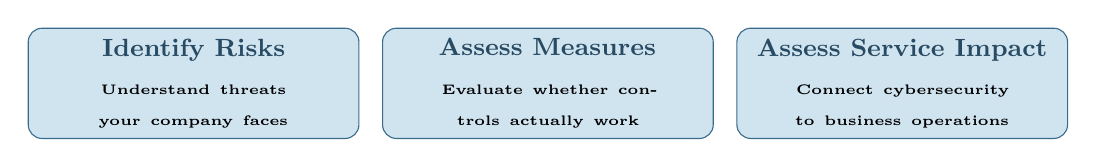
\begin{tikzpicture}[
  comp/.style={rectangle, rounded corners=5pt, draw=nisd2mid, fill=nisd2light,
    minimum width=4.2cm, minimum height=1.4cm, align=center,
    font=\small\bfseries, text width=3.8cm}
]
\node[comp] (c1) at (-4.5, 0) {\textcolor{nisd2blue}{Identify Risks}\\[3pt]\tiny Understand threats your company faces};
\node[comp] (c2) at (0, 0) {\textcolor{nisd2blue}{Assess Measures}\\[3pt]\tiny Evaluate whether controls actually work};
\node[comp] (c3) at (4.5, 0) {\textcolor{nisd2blue}{Assess Service Impact}\\[3pt]\tiny Connect cybersecurity to business operations};
\end{tikzpicture}
\par\smallskip\noindent{\small\textit{Three competence areas required by Article 20(2). Covering only one or two fails the standard.}}
\end{center}

\textbf{Frequency:} ``Regular'' in Germany means at minimum every three years; BSI recommends annual. The training duty is \textbf{personal and non-delegable}.

\begin{keytakeaways}
\begin{enumerate}
  \item Training must cover all three competence areas covering only one or two fails the standard.
  \item Minimum every three years in Germany; annual recommended by the BSI. Non-delegable.
  \item The auditor judges sufficiency based on content covered, time spent, and documentation, not on which body issued a certificate.
\end{enumerate}
\end{keytakeaways}

%  LESSON 1.7 
\section{\lessontag{1.7}Personal Liability Under Your Country's Corporate Law}

Your company gets fined €10 million for a NIS2 failure. Your supervisory board meets the next morning. The first item: whether to sue you, personally, for those €10 million, and under your country's corporate law, they are allowed to.

\begin{warningbox}
In many EU countries, including Germany, the \textbf{reverse burden of proof} applies to director liability. The company does not have to prove you were careless. \textbf{You have to prove you were careful.}

Your defence: the dated sign-off, the training record, the meeting minutes, the risk register with your signature. Without them, you are arguing from an empty file.
\end{warningbox}

\begin{keytakeaways}
\begin{enumerate}
  \item The EU directive creates the duty; your national corporate law turns it into a personal financial claim your own company can bring against you.
  \item In Germany, the burden of proof runs against the director: you must prove due care.
  \item Documentation is your only defence.
\end{enumerate}
\end{keytakeaways}

%  LESSON 1.8 
\section{\lessontag{1.8}The Business Judgment Rule Does Not Protect You}

The Business Judgment Rule protects directors from personal liability for \emph{business decisions} made in good faith. It does \textbf{not} cover statutory duties.

The principle is called the \textbf{duty of legality}: a director must comply with applicable law. No business judgment is permitted about \emph{whether} to follow a legal duty. ``I made a reasonable business decision not to fully implement Article~21'' is not a valid defence.

\begin{casestudy}{SolarWinds (2023)}
The SEC charged the CISO of SolarWinds personally after a supply-chain breach. The claim relied on internal documents, Slack messages, risk reports, showing a gap between external disclosures and internal reporting. Three lessons directly applicable to NIS2:
\begin{enumerate}
  \item Internal risk reports named control gaps that leadership did not close.
  \item The company's external security posture diverged from internal reports.
  \item Risk information was not reaching leadership in actionable form.
\end{enumerate}
\end{casestudy}

\begin{keytakeaways}
\begin{enumerate}
  \item The Business Judgment Rule protects commercial decisions, not compliance with law Article~20 and Article~21 create statutory duties under the duty of legality.
  \item ``I made a reasonable business decision not to implement the measure'' is not a valid defence.
  \item Internal documents, risk reports, assessments, meeting minutes, are what the regulator uses to prove you knew about the gap.
\end{enumerate}
\end{keytakeaways}

%  LESSON 1.9 
\section{\lessontag{1.9}The Ten Measures - Overview}

There are \textbf{ten} of them. Not eight. Not twelve. Having eight out of ten is not a passing grade.

\begin{center}
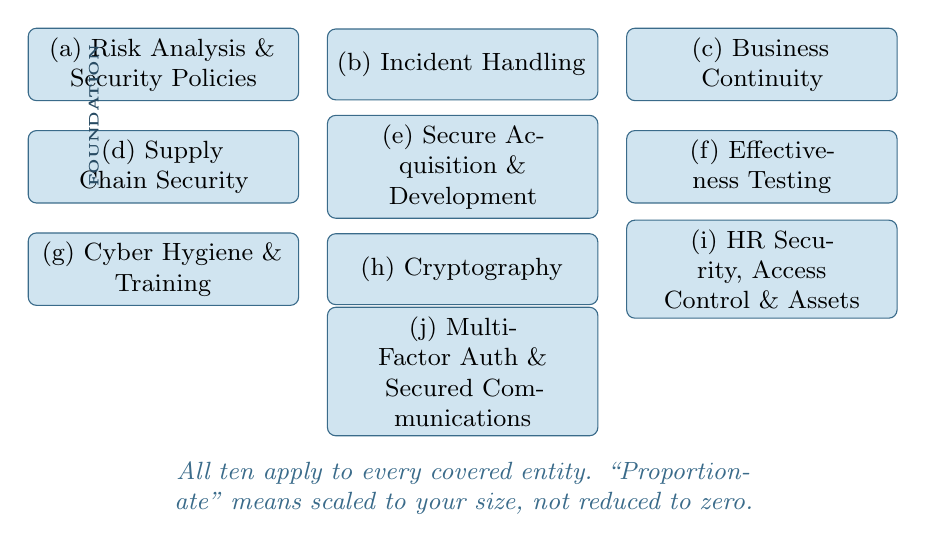
\begin{tikzpicture}[
  measure/.style={rectangle, rounded corners=3pt, draw=nisd2mid,
    fill=nisd2light, minimum width=3.4cm, minimum height=0.9cm,
    align=center, font=\small, text width=3.2cm}
]
% Row 1
\node[measure] (m1) at (0, 5.5)    {(a) Risk Analysis \&\\Security Policies};
\node[measure] (m2) at (3.8, 5.5)  {(b) Incident Handling};
\node[measure] (m3) at (7.6, 5.5)  {(c) Business Continuity};
% Row 2
\node[measure] (m4) at (0, 4.2)    {(d) Supply Chain Security};
\node[measure] (m5) at (3.8, 4.2)  {(e) Secure Acquisition \&\\Development};
\node[measure] (m6) at (7.6, 4.2)  {(f) Effectiveness Testing};
% Row 3
\node[measure] (m7) at (0, 2.9)    {(g) Cyber Hygiene \&\\Training};
\node[measure] (m8) at (3.8, 2.9)  {(h) Cryptography};
\node[measure] (m9) at (7.6, 2.9)  {(i) HR Security, Access\\Control \& Assets};
% Row 4 (centred)
\node[measure] (m10) at (3.8, 1.6)  {(j) Multi-Factor Auth \&\\Secured Communications};

% Proportionality note
\node[below=0.2cm of m10, font=\small\itshape, text=nisd2mid, text width=10cm, align=center]
  {All ten apply to every covered entity. ``Proportionate'' means scaled to your size, not reduced to zero.};

% Bracket labels
\node[left=0.3cm of m1, font=\tiny\bfseries, rotate=90, text=nisd2blue, anchor=south] at (-0.4, 4.85) {FOUNDATION};
\end{tikzpicture}
\end{center}

Each category needs three layers: \textbf{technical}, \textbf{operational}, and \textbf{organisational}. A firewall without a policy is incomplete. A policy without a working process is incomplete.

\begin{keytakeaways}
\begin{enumerate}
  \item There are ten specific categories in Article~21(2) all ten apply to every covered entity, none are optional.
  \item ``Proportionate'' means scaled to your size and risk exposure, not reduced to zero; a small company still needs all ten.
  \item The common failure: most measures in good shape but one or two missing entirely. The missing ones are the violation.
\end{enumerate}
\end{keytakeaways}

%  LESSONS 1.10–1.12 CONDENSED 
\section{\lessontag{1.10}All-Hazards Approach and State of the Art}

Article~21(1) requires risk management ``based on an all-hazards approach that aims to protect network and information systems and the \textbf{physical environment} of those systems from incidents.''

\textbf{All-hazards} means: cyber attacks, physical break-ins, fires, floods, power outages, supplier failures, insider threats, and human error  all in scope. A risk assessment that only lists cyber attacks does not meet the standard.

\textbf{State of the art} means current best practice as recognised by published standards at the \emph{time of audit}, not when you first implemented. Controls need a review cycle: \textbf{at minimum annually.}

\begin{keytakeaways}
\begin{enumerate}
  \item All-hazards covers everything that can hit the systems, not just hackers.
  \item State of the art is measured against standards current at the time of audit, not when you first implemented.
  \item Your controls need a review cycle, the rule is not ``implement once'' but ``keep current.''
\end{enumerate}
\end{keytakeaways}

\begin{quizbox}
\setcounter{quizq}{0}
\quizquestion{What does the all-hazards approach require?}{
  \item Protection only against cyber attacks
  \item \correct{Protection against every threat, cyber attacks, physical threats, environmental events, supplier failures, insider threats, and human error}
  \item Protection only against threats that have occurred before
  \item Protection only against threats listed in the risk register
}
\quizquestion{Against what point in time does the auditor judge whether controls meet ``state of the art''?}{
  \item When the controls were first implemented
  \item \correct{The standards current at the time of the audit}
  \item The date the NIS2 Directive entered into force
  \item When the company was first founded
}
\end{quizbox}

\section{\lessontag{1.11}The Reporting Cascade and Significant Incidents}

\begin{center}
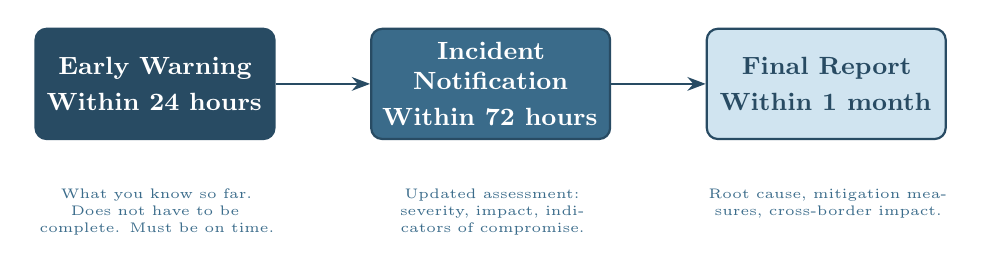
\begin{tikzpicture}[
  reportstep/.style={rectangle, rounded corners=4pt, draw=nisd2blue, thick,
    minimum width=3.0cm, minimum height=1.4cm, align=center,
    font=\small\bfseries, text width=2.8cm},
  arrow/.style={-{Stealth}, thick, color=nisd2blue}
]
\node[reportstep, fill=nisd2blue, text=white] (ew) at (0,0)
  {Early Warning\\[2pt]\small Within \textbf{24 hours}};
\node[reportstep, fill=nisd2mid, text=white, right=1.2cm of ew] (in)
  {Incident Notification\\[2pt]\small Within \textbf{72 hours}};
\node[reportstep, fill=nisd2light, text=nisd2blue, right=1.2cm of in] (fr)
  {Final Report\\[2pt]\small Within \textbf{1 month}};

\draw[arrow] (ew) -- (in);
\draw[arrow] (in) -- (fr);

\node[below=0.5cm of ew, font=\tiny, text=nisd2mid, text width=3cm, align=center]
  {What you know so far. Does not have to be complete. Must be on time.};
\node[below=0.5cm of in, font=\tiny, text=nisd2mid, text width=3cm, align=center]
  {Updated assessment: severity, impact, indicators of compromise.};
\node[below=0.5cm of fr, font=\tiny, text=nisd2mid, text width=3cm, align=center]
  {Root cause, mitigation measures, cross-border impact.};
\end{tikzpicture}
\par\smallskip\noindent{\small\textit{Late reporting is a separate sanctionable violation.}}
\end{center}

A significant incident under CIR 2024/2690 is triggered if \emph{any one} of: financial loss \textgreater{} €500,000 or 5\% of turnover (whichever is lower), trade secret exfiltration, death or serious health damage, or malicious unauthorised access causing severe disruption.

\textbf{Article 4 recurring rule:} Two or more incidents with the same root cause within six months that together cross the threshold = one significant incident. Track root causes.

\begin{keytakeaways}
\begin{enumerate}
  \item Significant incident threshold: €500,000 or 5\% turnover (whichever is lower), trade secrets, death, serious health, or malicious access causing severe disruption.
  \item Two or more same-root-cause incidents within six months that together cross the threshold count as one significant incident.
  \item The cascade: 24h (early warning), 72h (notification), 1 month (final report)  late reporting is its own separate fine.
\end{enumerate}
\end{keytakeaways}

\section{\lessontag{1.12}The Customer Notification Duty}

Two separate customer-facing duties:

\begin{itemize}
  \item \textbf{Article~23(2)  self-executing:} When a significant incident is likely to adversely affect customers, notify them without undue delay and tell them what protective measures they can take. No regulator order needed.
  \item \textbf{Article~36  regulator-ordered:} The regulator can instruct customer notification in the public interest.
\end{itemize}

A company that waits for a regulator order when its customers face an active threat has already failed Article~23(2).

\begin{keytakeaways}
\begin{enumerate}
  \item Article~23(2) is self-executing, when customers face an ongoing threat, notify them without undue delay and tell them what they can do. No regulator order needed.
  \item Article~36 is a separate power, but waiting for it when customers face an active threat already breaches Article~23(2).
  \item Have a pre-drafted customer notification template and a defined approval chain before an incident happens.
\end{enumerate}
\end{keytakeaways}

% ============================================================
%  CHAPTER 2: RISK AND THE 10 MEASURES
% ============================================================

\chapter{Risk and the 10 Measures}

\begin{moduleintro}
\textbf{Module 2 - 15 Lessons}

This module covers the risk management framework behind Article~21 and walks through each of the ten measures in detail. By the end, you will be able to walk the ten measures with your CISO and ask the right questions about each one.
\end{moduleintro}

\section{\lessontag{2.1}Risk = Likelihood $\times$ Impact}

Article~21(1) requires ``appropriate and proportionate'' measures to manage cybersecurity risks. How much you spend on security has to match how exposed you are.

\begin{center}
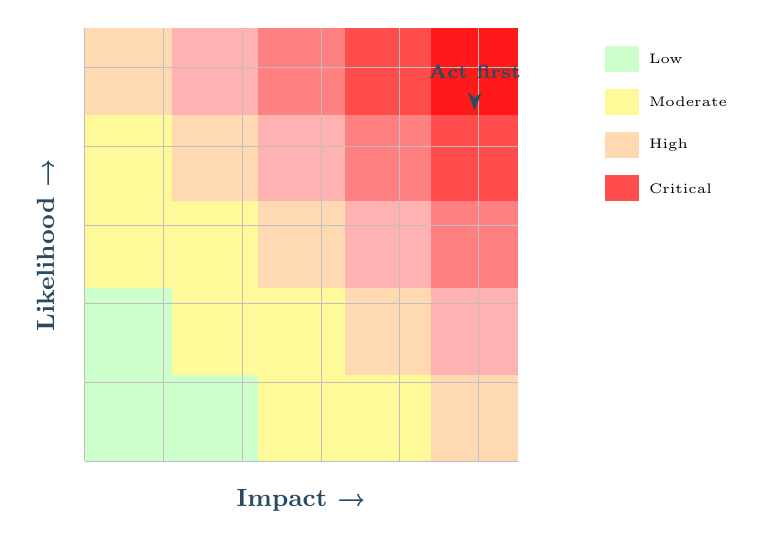
\begin{tikzpicture}
% Risk matrix
\def\sz{1.1}
% Cells
\fill[green!20] (0,0) rectangle (\sz,\sz);
\fill[green!20] (\sz,0) rectangle (2*\sz,\sz);
\fill[yellow!40] (2*\sz,0) rectangle (3*\sz,\sz);
\fill[yellow!40] (3*\sz,0) rectangle (4*\sz,\sz);
\fill[orange!30] (4*\sz,0) rectangle (5*\sz,\sz);

\fill[green!20] (0,\sz) rectangle (\sz,2*\sz);
\fill[yellow!40] (\sz,\sz) rectangle (2*\sz,2*\sz);
\fill[yellow!40] (2*\sz,\sz) rectangle (3*\sz,2*\sz);
\fill[orange!30] (3*\sz,\sz) rectangle (4*\sz,2*\sz);
\fill[red!30] (4*\sz,\sz) rectangle (5*\sz,2*\sz);

\fill[yellow!40] (0,2*\sz) rectangle (\sz,3*\sz);
\fill[yellow!40] (\sz,2*\sz) rectangle (2*\sz,3*\sz);
\fill[orange!30] (2*\sz,2*\sz) rectangle (3*\sz,3*\sz);
\fill[red!30] (3*\sz,2*\sz) rectangle (4*\sz,3*\sz);
\fill[red!50] (4*\sz,2*\sz) rectangle (5*\sz,3*\sz);

\fill[yellow!40] (0,3*\sz) rectangle (\sz,4*\sz);
\fill[orange!30] (\sz,3*\sz) rectangle (2*\sz,4*\sz);
\fill[red!30] (2*\sz,3*\sz) rectangle (3*\sz,4*\sz);
\fill[red!50] (3*\sz,3*\sz) rectangle (4*\sz,4*\sz);
\fill[red!70] (4*\sz,3*\sz) rectangle (5*\sz,4*\sz);

\fill[orange!30] (0,4*\sz) rectangle (\sz,5*\sz);
\fill[red!30] (\sz,4*\sz) rectangle (2*\sz,5*\sz);
\fill[red!50] (2*\sz,4*\sz) rectangle (3*\sz,5*\sz);
\fill[red!70] (3*\sz,4*\sz) rectangle (4*\sz,5*\sz);
\fill[red!90] (4*\sz,4*\sz) rectangle (5*\sz,5*\sz);

% Grid lines
\draw[gray!50, thin] (0,0) grid (5*\sz, 5*\sz);

% "Act first here" label
\node[font=\scriptsize\bfseries, text=nisd2blue] at (4.5*\sz, 4.5*\sz) {Act first};
\draw[-{Stealth}, thick, nisd2blue] (4.5*\sz, 4.2*\sz) -- (4.5*\sz, 4.05*\sz);

% Axis labels
\node[rotate=90, font=\small\bfseries, text=nisd2blue] at (-0.5, 2.5*\sz) {Likelihood →};
\node[font=\small\bfseries, text=nisd2blue] at (2.5*\sz, -0.5) {Impact →};

% Legend
\fill[green!20] (6*\sz, 4.5*\sz) rectangle (6.4*\sz, 4.8*\sz); \node[right, font=\tiny] at (6.4*\sz, 4.65*\sz) {Low};
\fill[yellow!40] (6*\sz, 4.0*\sz) rectangle (6.4*\sz, 4.3*\sz); \node[right, font=\tiny] at (6.4*\sz, 4.15*\sz) {Moderate};
\fill[orange!30] (6*\sz, 3.5*\sz) rectangle (6.4*\sz, 3.8*\sz); \node[right, font=\tiny] at (6.4*\sz, 3.65*\sz) {High};
\fill[red!70] (6*\sz, 3.0*\sz) rectangle (6.4*\sz, 3.3*\sz); \node[right, font=\tiny] at (6.4*\sz, 3.15*\sz) {Critical};
\end{tikzpicture}
\par\smallskip\noindent{\small\textit{The risk matrix. The top-right corner, high likelihood, high impact, is where the management body's job begins.}}
\end{center}

If you sign off on cybersecurity measures without understanding the risk picture behind them, your signature is uninformed, and an uninformed sign-off does not protect you under Article~20(1).

\begin{keytakeaways}
\begin{enumerate}
  \item Every risk decision under NIS2 comes down to two questions, how likely and how bad.
  \item The top-right corner of the matrix is where the management body's job begins.
  \item The risk register turns the budget argument from opinion into evidence, ask to see it, and check whether the dates are current.
\end{enumerate}
\end{keytakeaways}

\section{\lessontag{2.2}What Is an Asset?}

\begin{casestudy}{Equifax (2017)}
Equifax had a patch for a critical vulnerability. They applied it to every server except one. That one server was not on any list. 147 million records were stolen through it. The root cause was not the missing patch  it was the missing inventory entry.
\end{casestudy}

An asset is \textbf{anything the business depends on to operate}: servers, laptops, customer databases, cloud subscriptions, buildings, suppliers, employees with critical knowledge, and key business processes. The full list is called the \textbf{asset inventory}, and it must be kept current.

The auditor asks for the inventory \emph{before} they ask for policies, the risk matrix, or anything else, because every other control is only as complete as the list it covers.

\begin{actionbox}
``Show me the asset inventory. When was it last updated, and does it include cloud subscriptions and contractor access?''
If the answer covers only servers and laptops, the inventory is incomplete.
\end{actionbox}

\section{\lessontag{2.3}Risk Treatment Options and Risk Appetite}

Four options for every risk: \textbf{Avoid, Mitigate, Transfer, Accept.} For NIS2 entities, mitigate is the workhorse, transfer and accept are rarely defensible for serious risks.

\begin{warningbox}
CIR 2024/2690, Annex 2.1.1: ``Risk assessment results and residual risks shall be accepted by management bodies.'' Your signature, dated, on the register or acceptance sheet. \textbf{The CIR anchors the entire risk-management chain on this signature: without it, the rest is treated as unapproved.}
\end{warningbox}

The \textbf{risk appetite} the level of risk the company is willing to live with overall, is the CEO's boundary to set, not the CISO's. Without it, every risk treatment decision becomes an argument.

\section{\lessontag{2.4}Why Risk Management Is Continuous}

Article~21 does not say ``conduct a risk analysis.'' It says you must take ``appropriate and proportionate'' measures, \textbf{present tense, continuously}. Risk management is a cycle, not a project.

Minimum review cadence: \textbf{annual} (BSI Standard 200-1, Section 7.4). Plus any time a trigger fires: major incident, significant business change, new vulnerability disclosure, regulatory change, or audit finding.

\section{\lessontag{2.5}The CIA Triad and Business Impact}

\begin{center}
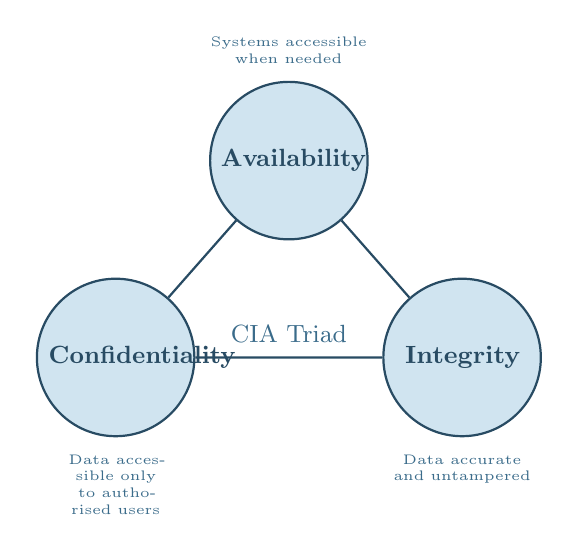
\begin{tikzpicture}[
  comp/.style={circle, draw=nisd2blue, thick, minimum size=2.0cm,
    align=center, font=\small\bfseries, text width=1.7cm}
]
\node[comp, fill=nisd2light] (C) at (-2.2, 0) {\textcolor{nisd2blue}{Confidentiality}};
\node[comp, fill=nisd2light] (I) at (2.2, 0)  {\textcolor{nisd2blue}{Integrity}};
\node[comp, fill=nisd2light] (A) at (0, 2.5)  {\textcolor{nisd2blue}{Availability}};
\node[font=\small, text=nisd2mid] at (0, 0.3) {CIA Triad};
\draw[nisd2blue, thick] (C) -- (I) -- (A) -- (C);
\node[below=0.1cm of C, font=\tiny, text=nisd2mid, align=center, text width=2cm] {Data accessible only\\to authorised users};
\node[below=0.1cm of I, font=\tiny, text=nisd2mid, align=center, text width=2cm] {Data accurate\\and untampered};
\node[above=0.1cm of A, font=\tiny, text=nisd2mid, align=center, text width=2cm] {Systems accessible\\when needed};
\end{tikzpicture}
\end{center}

The \textbf{Business Impact Analysis (BIA)} translates CIA categories into business numbers: recovery targets and business consequences. The CEO's role is not to calculate the BIA  it is to \emph{validate the business assumptions in it}.

\section{\lessontag{2.6}Measure 1  Risk Analysis and Information Security Policies}

The CIR requires \textbf{eleven distinct policies}:

\begin{center}
\begin{tabular}{@{}ll@{}}
\toprule
\textbf{\#} & \textbf{Required Policy} \\
\midrule
1 & Information security policy (top-level  \textbf{your signature, your name}) \\
2 & Risk management \\
3 & Incident handling \\
4 & Supply chain security \\
5 & Security testing \\
6 & Effectiveness assessment \\
7 & Cryptography \\
8 & Access control \\
9 & Privileged accounts \\
10 & Information and asset handling \\
11 & Removable media \\
\bottomrule
\end{tabular}
\end{center}

Three CIR Annex policies that are easy to miss when adapting a generic ISO set: \textbf{security testing, privileged accounts, removable media.}

The top-level policy must carry your personal signature and be published in your name. It must be reviewed \textbf{annually} with a dated management body approval.

\begin{quizbox}
\setcounter{quizq}{0}
\quizquestion{How many distinct policies does the CIR require for Measure 1?}{
  \item One comprehensive security policy
  \item Five core policies
  \item \correct{Eleven (one top-level plus ten topic-specific)}
  \item Three (risk, incident, access)
}
\quizquestion{Which three CIR Annex topic-specific policies does this lesson call out as worth double-checking?}{
  \item Risk management, incident handling, access control
  \item \correct{Security testing, privileged accounts, removable media}
  \item Cryptography, supply chain, effectiveness assessment
  \item Backup, disaster recovery, crisis management
}
\end{quizbox}

\section{\lessontag{2.7}Measure 2 - Incident Handling}

Five parts to an incident response plan: \textbf{detection, classification, response, recovery, lessons learned.}

CEO-specific entries in the plan (must be pre-assigned by name):
\begin{itemize}
  \item Declaring a crisis
  \item Authorising emergency spending
  \item Approving external communication to customers and the regulator
  \item Deciding whether to pay a ransom
\end{itemize}

The plan must be tested. A \textbf{tabletop exercise}, a paper rehearsal against a scenario, conducted less than 12 months ago, with documented changes as a result.

\section{\lessontag{2.8}Measure 3 - Business Continuity}

\begin{casestudy}{Maersk (2017)}
NotPetya malware wiped Maersk's global IT in under two hours. Recovery cost: ~€300 million. The only reason it took 10 days instead of months: one backup happened to be offline due to a power cut in Ghana. Luck is not a control.
\end{casestudy}

Three components: \textbf{backup management} (tested, stored separately), \textbf{disaster recovery} (RTO and RPO defined and verified by actual testing), \textbf{crisis management} (named team, pre-assigned authority, exercised annually).

\begin{definitionbox}{RTO and RPO}
\textbf{RTO (Recovery Time Objective):} How quickly must this system be back up after an incident? \\
\textbf{RPO (Recovery Point Objective):} How much data can the company afford to lose, measured in time?
\end{definitionbox}

You must attend the annual crisis exercise. BSI DER.4 names the management body in nine of sixteen requirements, absence is an audit finding.

\section{\lessontag{2.9}Measure 4 - Supply Chain Security}

\begin{casestudy}{SolarWinds (2020)}
A routine software update to 18,000 customers contained a back door planted by attackers. Every customer had to treat it as their own incident, not their supplier's.
\end{casestudy}

``Supplier'' under NIS2 means \textbf{anyone with access to your systems or data}, from cloud provider to the cleaning company with a key to the server room.

Four things required for each supplier:
\begin{enumerate}
  \item Supplier inventory entry
  \item Risk classification
  \item Contractual clauses: incident notification, audit rights, security baseline
  \item Periodic review (questionnaire, certificate, or audit)
\end{enumerate}

If your supplier is breached and your customers' data leaks, the reporting duty under Article~23 and the customer notification duty under Article~36 both land on \textbf{you}, not the supplier.

\section{\lessontag{2.10}Measure 5 - Acquisition, Development, and Maintenance}

Three duties: \textbf{secure acquisition} (security requirements in every purchase), \textbf{secure development} (documented standard if you write software), \textbf{vulnerability handling} (patch SLAs exist on paper, results tracked quarterly).

The single most important operational evidence: \textbf{a written patch SLA and a quarterly report on whether you are meeting it.}

\begin{actionbox}
``What is our patch SLA on critical vulnerabilities, and in the last quarter, on what percentage of systems did we meet it?''
\end{actionbox}

\section{\lessontag{2.11}Measure 6 - Effectiveness Assessment}

The \textbf{annual management review} is a discrete obligation under BSI Standard 200-1, Section 7.4. It must produce a \textbf{signed protocol} with:
\begin{itemize}
  \item Status of the security programme since last review
  \item Whether previous decisions were carried out
  \item New threats, resource needs, residual risks accepted
\end{itemize}

The auditor's first question on Measure 6: ``Show me the protocol of your last annual management review, and show me that the follow-up actions were closed.'' Without a dated, signed protocol, the entire measure fails the audit.

\section{\lessontag{2.12}Measure 7 - Cyber Hygiene and Training}

Two halves: \textbf{cyber hygiene} (daily basics: strong passwords, MFA, regular updates, backups, cautious links) and \textbf{training} (scheduled programme).

Training applies to:
\begin{itemize}
  \item All staff: annual awareness training
  \item Technical/high-risk roles: role-specific training
  \item Management body: its own programme under Article~20(2)
\end{itemize}

One generic e-learning course for the whole company does not satisfy this requirement. \textbf{Phishing simulations} with follow-up training for anyone who clicks are part of the programme.

A CEO who skips the phishing simulation or exempts themselves from the awareness programme has created a \textbf{personal audit finding} under BSI Standard 200-1 Principle 6.

\section{\lessontag{2.13}Measure 8 - Cryptography}

The cryptography policy must cover \textbf{encryption at rest} and \textbf{encryption in transit}, and must name where each applies.

Reference \textbf{BSI TR-02102} in the policy rather than hardcoding algorithm names, the guideline is updated as research evolves, so the policy stays current automatically.

Key management is where cryptography fails in practice. Ask: Where are the keys stored? If the answer is ``on the same server as the data,'' that is a gap. Who can access them? When were they last rotated?

\section{\lessontag{2.14}Measure 9 - HR Security, Access Control, and Asset Management}

The most common audit finding: \textbf{the leaver step}, a former employee still holding a live VPN login or active administrator account weeks after departure.

The \textbf{joiner-mover-leaver process}: the three handovers between HR and IT. If any one is broken, Measure~9 is broken. For critical roles, access revocation happens the moment the termination is decided, not the day the person walks out.

\textbf{Privileged accounts} need a dedicated policy with stronger controls and their own review cadence (CIR Annex 11.3).

\section{\lessontag{2.15}Measure 10 - Multi-Factor Authentication and Secured Communications}

MFA is effectively mandatory for four categories:

\begin{center}
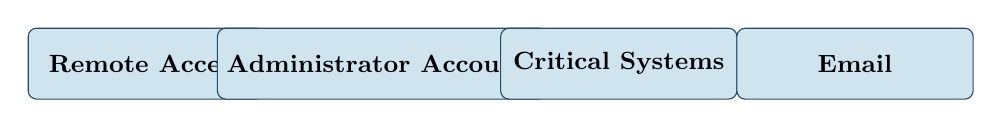
\begin{tikzpicture}[
  box/.style={rectangle, rounded corners=3pt, draw=nisd2blue, fill=nisd2light,
    minimum width=3cm, minimum height=0.9cm, align=center, font=\small\bfseries}
]
\node[box] at (-4.5, 0) {Remote Access};
\node[box] at (-1.5, 0) {Administrator Accounts};
\node[box] at (1.5, 0)  {Critical Systems};
\node[box] at (4.5, 0)  {Email};
\end{tikzpicture}
\end{center}

\textbf{Secured emergency communications:} An out-of-band channel that works when normal systems are compromised. If the crisis plan relies on email and email is down, the plan fails at the worst moment.

\textbf{Lead-by-example (BSI Standard 200-1 Principle 6):} Your own account is the first one the auditor checks. A CEO who approved MFA but exempted their own login has created a personal finding.

\begin{actionbox}
Check your own email account today, is MFA turned on? If not, turn it on. Ten minutes.
\end{actionbox}

\begin{quizbox}
\setcounter{quizq}{0}
\quizquestion{For which four categories is MFA effectively mandatory?}{
  \item Personal email, social media, personal banking, and personal devices
  \item \correct{Remote access, administrator accounts, critical systems, and email}
  \item Marketing tools, HR systems, accounting software, and the company website
  \item Board meetings, investor portals, press releases, and internal chat
}
\quizquestion{What is the CEO's own account the first one the auditor checks for MFA?}{
  \item Because the CEO's account contains the most sensitive data
  \item \correct{Because BSI Standard 200-1 Principle 6 requires the management body to personally follow the security controls they approved}
  \item Because the auditor starts alphabetically
  \item Because the regulator specifically named the CEO role in Article~21
}
\end{quizbox}

% ============================================================
%  CHAPTER 3: DECISION SUPPORT
% ============================================================

\chapter{Decision Support}

\begin{moduleintro}
\textbf{Module 3 - 11 Lessons}

This module covers the governance decisions only you can make: what to sign, when to re-sign, how to run an audit, and how to handle the hardest scenarios, ransomware, supplier breaches, and pre-audit gap discovery.
\end{moduleintro}

\section{\lessontag{3.1}The Questions Every CEO Must Answer}

The BSI has published a list of structured questions every management body must be able to answer. These are the most concrete practical test of Article~20(2) any EU regulator has published.

\begin{center}
\begin{tabular}{@{}p{0.3cm}p{10.5cm}@{}}
\toprule
\multicolumn{2}{l}{\textbf{Foundation (5 questions)}} \\
\midrule
1 & Do I know whether my company falls under NIS2 and understand the scope of the law? \\
2 & Do our risk-management measures meet the law's requirements, and are they documented? \\
3 & Can I classify a significant incident correctly and report it on time? \\
4 & Are we registered correctly with the regulator, and do we keep that registration current? \\
5 & Do I understand my personal duties, training requirements, liability, and the sanctions I face? \\
\midrule
\multicolumn{2}{l}{\textbf{The Ten Mandatory Measures (10 sub-questions)}} \\
\midrule
6.1 & Is our risk analysis up to date and aligned with current threats? \\
6.2 & Do we have a tested incident response plan? \\
6.3 & Can we recover from backup, and is our crisis management tested? \\
6.4 & Is supplier security checked and actively managed? \\
6.5 & Is security built into how we acquire, develop, and maintain systems? \\
6.6 & Do we measure the effectiveness of our security controls? \\
6.7 & Do we run cyber hygiene programmes and staff training? \\
6.8 & Do we use cryptography and encryption where required? \\
6.9 & Do we manage personnel security, access control, and asset management? \\
6.10 & Do we use multi-factor authentication and secured communications? \\
\midrule
\multicolumn{2}{l}{\textbf{Deeper Checks (4 questions)}} \\
\midrule
7 & Does our risk analysis cover all assets, threats, vulnerabilities, and types of damage  including reputational and regulatory harm? \\
8 & Do we evaluate how each risk affects availability, integrity, and confidentiality, as well as financial stability? \\
9 & Do we account for sector-specific requirements and our most critical business processes? \\
10 & Do we run scenario exercises, and have I personally participated in one? \\
\bottomrule
\end{tabular}
\end{center}

\begin{actionbox}
Print this list and go through it with your CISO. Rate each: \textbf{confident / with help / cannot answer.} Every question in the third column is a gap your training must close.
\end{actionbox}

\section{\lessontag{3.2}Sign-Off in Practice}

Four questions to ask before you sign any security document:

\begin{enumerate}
  \item \textbf{``Show me the risk analysis this policy refers to, when was it last updated?''}
  \item \textbf{``What has changed since the last version I signed?''}
  \item \textbf{``Has the budget to implement these measures been approved?''} A policy that promises controls the company has not funded is a policy the regulator will use against you.
  \item \textbf{``Who are the named people responsible for each measure, and do they know they are named?''} Unassigned measures are intentions, not controls.
\end{enumerate}

The management body decides \textbf{what and why}. The CISO decides \textbf{how}. An uninformed signature is legally void in most EU jurisdictions, and in court it works against you, not for you.

\section{\lessontag{3.3}When to Re-Sign-Off}

Annual is the floor. Six types of events force re-sign-off before the annual cycle:

\begin{enumerate}
  \item Change in leadership
  \item Significant change in the business (acquisition, new geography, new product)
  \item Major incident that exposed a gap
  \item Regulatory change
  \item Audit finding requiring remediation
  \item Material change in the supplier base
\end{enumerate}

Every re-sign-off documents three things: the \textbf{trigger event}, the \textbf{changes to the measures}, and the \textbf{new signature}.

\section{\lessontag{3.4}Red Flags in Your Team's Sign-Off Process}

Nine sentences that should make you put the pen down:

\begin{center}
\renewcommand{\arraystretch}{1.3}
\begin{tabularx}{\linewidth}{@{}X X@{}}
\toprule
\textbf{Red Flag} & \textbf{Your Response} \\
\midrule
``We have always done it this way.'' & ``Show me the version history.'' \\
``Sign here, it is just a formality.'' & ``If it is a formality, why does it need my signature?'' \\
``Our IT department handles this.'' & ``I am leadership. That makes me the person who must understand it.'' \\
``We cannot afford that control.'' & ``Show me the risk assessment that says this is an acceptable residual risk.'' \\
``We have never had a problem.'' & ``That is not an answer. Show me the current test results.'' \\
``It is documented, but you cannot access it.'' & ``Then I will wait until I can read it.'' \\
``Just trust the auditor.'' & ``The auditor has a job and I have a job. This is mine.'' \\
``We will fix it after the audit.'' & ``If it is known, it is already a finding. Fix it now and I will sign the fix.'' \\
``The previous CEO signed something similar.'' & ``The previous CEO is not signing this. I am.'' \\
\bottomrule
\end{tabularx}
\end{center}

The rule: \textbf{if the explanation feels faster than the document, the process is broken.} Refusing to sign costs hours. Signing blind costs years.

\section{\lessontag{3.5}What You Cannot Delegate - The Checklist}

Eleven non-delegable decisions, eleven signed artefacts:

\begin{enumerate}
  \item Approval of the cybersecurity risk-management measures (top-level security policy, signed in your name)
  \item \textbf{Formal acceptance of residual risks}, the single document most CEOs cannot produce
  \item Approval of the security budget
  \item Crisis declaration during a major incident
  \item The Article~23 reporting decision (your team drafts, you approve)
  \item Customer notification decisions under Article~36
  \item Authorisation of any extraordinary payment (ransomware, settlement, emergency vendor)
  \item Approval of all public statements during a crisis
  \item Engagement of external forensics or legal counsel in major incidents
  \item Resolution of conflicts between security and other business priorities when escalated
  \item The annual management review, formal, documented, signed, at least once a year
\end{enumerate}

\begin{warningbox}
The \textbf{residual risk acceptance} is the document the CIR anchors the entire risk-management chain on - without it, the rest is treated by the auditor as unapproved. Every risk the company has decided to live with must appear in the signed risk register with a rating, a description of what is being accepted, and a named owner with a review date. Your signature proves you personally reviewed what the company decided to live with.
\end{warningbox}

\section{\lessontag{3.6}CISO and Supervisory Board Reporting Lines}

\textbf{CIR 2024/2690, Annex 1.2.3:} ``At least one person shall report directly to the management bodies on matters of network and information system security.''

This is a \textbf{hard requirement}. A CISO reporting through IT or finance does not meet it, regardless of how competent the CISO is or how often they informally brief you.

\begin{center}
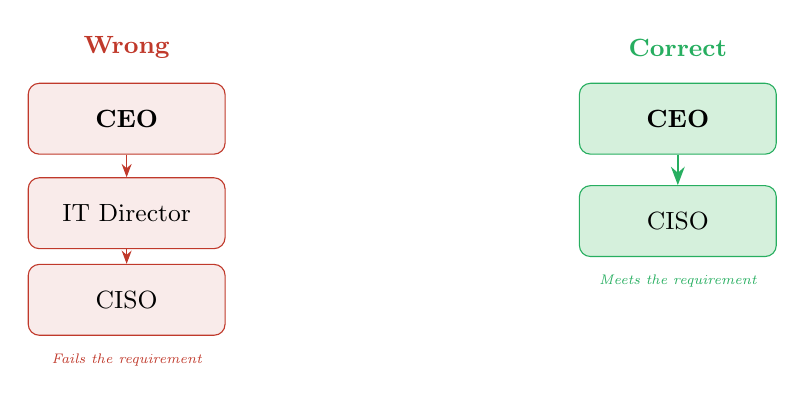
\begin{tikzpicture}[
  node/.style={rectangle, rounded corners=4pt, draw=nisd2blue,
    minimum width=2.5cm, minimum height=0.9cm, align=center, font=\small}
]
% Wrong
\node[node, fill=warningred!10, draw=warningred] (ceo1) at (-3.5, 2) {\textbf{CEO}};
\node[node, fill=warningred!10, draw=warningred] (it1) at (-3.5, 0.8) {IT Director};
\node[node, fill=warningred!10, draw=warningred] (ciso1) at (-3.5, -0.3) {CISO};
\draw[-{Stealth}, warningred] (ceo1.south) -- (it1.north);
\draw[-{Stealth}, warningred] (it1.south) -- (ciso1.north);
\node[below=0.1cm of ciso1, font=\tiny\itshape, text=warningred] {Fails the requirement};

% Right
\node[node, fill=correctgreen, draw=successgreen] (ceo2) at (3.5, 2) {\textbf{CEO}};
\node[node, fill=correctgreen, draw=successgreen] (ciso2) at (3.5, 0.7) {CISO};
\draw[-{Stealth}, successgreen, thick] (ceo2.south) -- (ciso2.north);
\node[below=0.1cm of ciso2, font=\tiny\itshape, text=successgreen] {Meets the requirement};

\node[font=\small\bfseries, text=warningred] at (-3.5, 2.9) {Wrong};
\node[font=\small\bfseries, text=successgreen] at (3.5, 2.9) {Correct};
\end{tikzpicture}
\end{center}

The budget and headcount do not have to change, only the line on the chart. Then schedule a recurring monthly meeting with a standing written agenda.

\section{\lessontag{3.7}What Happens During a Regulator Audit}

Seven documents form the backbone of your audit file:

\begin{enumerate}
  \item Article~21 policy set (all eleven policies)
  \item Signed risk register with residual risk acceptance
  \item Incident reports and lessons learned
  \item Training records (yours and your staff's)
  \item CISO-to-board reporting minutes
  \item Asset inventory
  \item Supplier contracts with the three critical clauses
\end{enumerate}

\begin{definitionbox}{Finding vs. Observation}
\textbf{Finding:} A non-conformance, something the law requires that you do not have. Triggers a remediation order with a deadline. \\
\textbf{Observation:} Falls below good practice but does not violate the law. Does not trigger an order.
\end{definitionbox}

If remediation is incomplete when the auditor returns: the regulator escalates to binding instructions, public disclosure, or fines.

\section{\lessontag{3.8}Scenario - Ransomware Hits Friday Afternoon}

\begin{casestudy}{Norsk Hydro (2019)}
LockerGoga ransomware shut down 40 production sites overnight. Cost: ~€60 million. Ransom paid: zero. The response worked because ransomware was already on the risk register, rated very likely / very serious, with a board-approved response plan.
\end{casestudy}

\textbf{Five decisions that belong to the CEO alone in the first 48 hours:}

\begin{enumerate}
  \item \textbf{Declare the crisis.} Only you can activate crisis procedures.
  \item \textbf{Authorise emergency spending.} Forensics vendors, external counsel, incident response firm.
  \item \textbf{Contain before you restore.} Restoring before forensics destroys the evidence chain.
  \item \textbf{File the 24-hour early warning.} File what you know. State what is uncertain.
  \item \textbf{Hold the line on payment.} Not now, and only after legal review of sanctions law.
\end{enumerate}

\section{\lessontag{3.9}Scenario - Supplier Breach Affecting Your Customer Data}

\begin{casestudy}{MOVEit (2023)}
Cl0p ransomware group exploited a zero-day in MOVEit file-transfer software. Within weeks, data from over 2,600 organisations was stolen. Breach at the supplier. Data belonged to the customers.
\end{casestudy}

\textbf{Five decisions in a supplier breach:}

\begin{enumerate}
  \item Force the facts: which systems were connected, what data was in transit, over what time period?
  \item Pull the contract: incident notification timelines, audit rights, indemnification.
  \item File your own report, the supplier's report does not cover you.
  \item Notify customers before the press does, under Article~36, hours after confirming exposure.
  \item Pursue contractual remedies \emph{calmly, after} the incident is handled.
\end{enumerate}

Speed of notification decides the reputational outcome. Customers judge you on how fast you told them, not on whose system was breached.

\section{\lessontag{3.10}Scenario - Phishing Success: Significant or Not?}

Four questions decide:

\begin{enumerate}
  \item Has the attacker \emph{used} the credentials?
  \item What did those credentials access? (email only vs finance vs customer databases)
  \item Was data exfiltrated?
  \item Does the financial impact cross the CIR thresholds?
\end{enumerate}

When genuinely uncertain, \textbf{file the early warning}. The regulator prefers ``we are not sure, here is what we know'' over silence. You cannot retroactively file one that should have been sent two days ago.

\section{\lessontag{3.11}Scenario - Pre-Audit Gap Discovery}

Three options when you find a gap two weeks before an audit:

\begin{center}
\begin{tabular}{@{}lll@{}}
\toprule
\textbf{Option} & \textbf{Action} & \textbf{Outcome} \\
\midrule
A & Hide it & Concealment found; cover-up is a separate violation \\
B & Fix it silently & Timestamps survive; looks like concealment \\
C & Fix it \textbf{and} disclose & \textcolor{successgreen}{Remediation order or warning, not a fine} \\
\bottomrule
\end{tabular}
\end{center}

In Option C: fix it immediately, document the discovery and timeline, then \textbf{you personally write to the auditor} before the audit  what was found, when, what was done, what the new controls look like.

\begin{keytakeaways}
\begin{enumerate}
  \item Finding your own gaps is the expected state - regulators distinguish between found-and-fixed versus hidden.
  \item Hiding a gap or quietly fixing it both fail when the audit trail tells the story.
  \item Good-faith disclosure, signed by the CEO, with the fix already in place, is the only option that strengthens your position.
\end{enumerate}
\end{keytakeaways}

% ============================================================
%  CHAPTER 4: PROTECTION
% ============================================================

\chapter{Protection}

\begin{moduleintro}
\textbf{Module 4 - 6 Lessons}

This module covers the protection layer around your personal exposure: why insurance is not a substitute for controls, what your D\&O policy actually covers, and how to handle the first 48 hours of a crisis.
\end{moduleintro}

\section{\lessontag{4.1}Insurance Is Not a Substitute for Controls}

\begin{casestudy}{Mondelez vs. Zurich Insurance (2017)}
Mondelez was hit by NotPetya malware and suffered ~\$100M in damage. Mondelez held a cyber policy with Zurich for that amount. Zurich refused the claim, arguing NotPetya was an act of war. Five years of litigation followed. Settlement: confidential.
\end{casestudy}

\textbf{Three things insurance does not remove:}
\begin{itemize}
  \item Regulatory fines under Article~32, most policies explicitly exclude them
  \item The manager ban under Article~34, no policy covers that
  \item The customer notification duty under Article~36, that lands on you regardless
\end{itemize}

The auditor does not accept an insurance certificate as evidence that you have implemented the ten measures. \textbf{Insurance pays after the incident. The auditor checks what you did before it.}

\section{\lessontag{4.2}D\&O Insurance - What It Covers and the Cyber Exclusions}

D\&O insurance was designed for \textbf{business judgment claims}, the allegation that a director made a bad business decision. NIS2 violations are \textbf{statutory duty breaches}, a different legal category that sits on the wrong side of the line most D\&O policies draw.

\begin{actionbox}
Three questions to ask your broker before every renewal:
\begin{enumerate}
  \item ``Does our current D\&O policy contain a cyber liability exclusion?''
  \item ``If I am personally named in a claim by the regulator under Article~32(5), does this policy pay for my legal defence?''
  \item ``What does the policy say about statutory duty breaches?''
\end{enumerate}
Get all three answers in writing, dated, and attached to the policy.
\end{actionbox}

\section{\lessontag{4.3}Cyber Insurance vs D\&O - Different Products, Different Coverage}

\begin{center}
\begin{tabular}{@{}lll@{}}
\toprule
\textbf{} & \textbf{Cyber Insurance} & \textbf{D\&O Insurance} \\
\midrule
\textbf{Named insured} & The company & The director \\
\textbf{Covers} & Forensics, notification, business interruption & Legal defence, settlements \\
\textbf{Designed for} & Cyber incident costs & Business judgment claims \\
\textbf{NIS2 personal fine?} & No & May exclude cyber claims \\
\bottomrule
\end{tabular}
\end{center}

The dangerous scenario: a director is sued personally for a cyber incident. The D\&O policy has an explicit cyber exclusion. The cyber policy does not cover individual directors. \textbf{The director is uncovered.}

Ask your broker to produce a one-page map of which claim scenarios are covered by which policy.

\section{\lessontag{4.4}Common Policy Exclusions to Read For}

\textbf{D\&O exclusions:}
\begin{itemize}
  \item The cyber liability exclusion (explicit or buried in broader language)
  \item Pre-existing condition exclusion
  \item Sanctions exclusion
  \item Acts-of-war exclusion (significantly broadened after Mondelez)
  \item Failure-to-maintain-security clause
  \item Late notification clause
\end{itemize}

\textbf{Cyber insurance exclusions:}
\begin{itemize}
  \item Pre-existing vulnerabilities and unpatched systems
  \item Acts-of-war / nation-state attack exclusion (Lloyd's tightened 2023)
  \item Sanctions law compliance
  \item Regulator fines and penalties \textbf{almost universally excluded}
\end{itemize}

\section{\lessontag{4.5}First 48 Hours of Crisis Communication}

\textbf{Four audiences, in order:} Internal first → Regulator second → Customers third → Public fourth.

Six decisions from the Maersk (NotPetya, 2017) case study:
\begin{enumerate}
  \item Designate \textbf{one spokesperson} in the first hour
  \item Issue a \textbf{holding statement within two hours} (acknowledges disruption, commits to update time)
  \item \textbf{Brief internal team} before any external statement
  \item \textbf{File the early warning} inside 24 hours
  \item \textbf{Notify affected customers} under Article~36
  \item Issue the \textbf{public statement last} after internal briefing, regulator report, and customer notification
\end{enumerate}

The CEO is rarely the spokesperson on television but is \textbf{always the final approver} of every external statement. Legal review is not optional.

\section{\lessontag{4.6}Ransomware Payment Decisions}

\begin{casestudy}{Colonial Pipeline (2021)}
Colonial Pipeline paid DarkSide ~\$4.5M in Bitcoin. The decryption tool was so slow they restored from backups anyway. The payment did not save time. The CEO stated a pre-agreed policy would have changed the decision. The company had no board-approved position on ransomware payment before the attack.
\end{casestudy}

\textbf{Three legal constraints on payment:}
\begin{enumerate}
  \item \textbf{Sanctions law} paying a sanctioned group is a violation even if you did not know. Attribution is often unclear in the first hours.
  \item \textbf{Corporate law} in Germany, a ransom payment where the decryption tool fails or backups were viable can trigger personal liability under Breach of Trust (§266 StGB).
  \item \textbf{Sector-specific rules} financial services, critical infrastructure, defence have additional restrictions.
\end{enumerate}

\textbf{Four steps before any payment:} CEO approval (non-delegable), legal review (sanctions + criminal law), law enforcement coordination, documentation in the incident record.

\textbf{The pre-agreed policy} is the deliverable: your incident response plan needs a board-approved position on ransomware payment, signed by the CEO. Roughly 60\% of payments yield usable decryption, often slower than a clean restore from backups.

\begin{keytakeaways}
\begin{enumerate}
  \item Paying does not guarantee recovery, roughly 60\% of payments yield usable decryption.
  \item Sanctions law bites regardless of intent, you cannot always identify the recipient.
  \item Make the payment decision before the attack, a pre-agreed policy signed by the CEO turns a crisis improvisation into a policy check.
\end{enumerate}
\end{keytakeaways}

\begin{quizbox}
\setcounter{quizq}{0}
\quizquestion{Why did Zurich refuse the Mondelez insurance claim?}{
  \item The policy had expired
  \item \correct{Zurich argued NotPetya was an act of war, triggering the acts-of-war exclusion}
  \item Mondelez had not paid its premium
  \item The damages exceeded the policy limit
}
\quizquestion{Which three consequences does insurance NOT remove?}{
  \item Business interruption, data loss, and reputational damage
  \item \correct{Regulatory fines, the manager ban, and the customer notification duty}
  \item Legal costs, forensic investigation, and incident response
  \item Staff turnover, supply chain disruption, and media coverage
}
\quizquestion{What should you do before any ransomware payment?}{
  \item Pay immediately to minimise disruption
  \item Consult the insurance broker and pay if covered
  \item \correct{CEO approval, legal review covering sanctions and criminal law, law enforcement coordination, and documentation}
  \item Wait for the regulator's guidance
}
\end{quizbox}

% ============================================================
%  CHAPTER 5: FINAL
% ============================================================

\chapter{Final}

\begin{moduleintro}
\textbf{Module 5 - 2 Lessons}

The 90-day action plan that turns knowledge into a defensible baseline, and what your Certificate of Completion means.
\end{moduleintro}

\section{\lessontag{5.1}Your First 90 Days After This Course}

Understanding is not compliance. The sequenced plan that turns knowledge into a defensible baseline:

\begin{center}
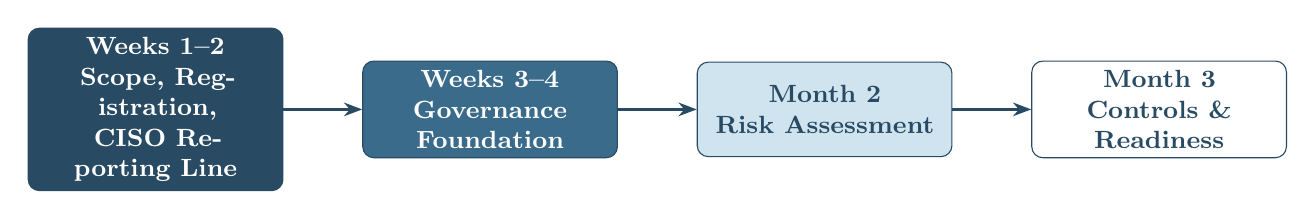
\begin{tikzpicture}[
  phase/.style={rectangle, rounded corners=4pt, draw=nisd2blue,
    minimum width=3.2cm, minimum height=1.2cm, align=center,
    font=\small\bfseries, text width=3.0cm},
  arrow/.style={-{Stealth}, thick, nisd2blue}
]
\node[phase, fill=nisd2blue, text=white] (w12) at (0, 4.5)
  {Weeks 1--2\\Scope, Registration,\\CISO Reporting Line};
\node[phase, fill=nisd2mid, text=white, right=1.0cm of w12] (w34)
  {Weeks 3--4\\Governance\\Foundation};
\node[phase, fill=nisd2light, text=nisd2blue, right=1.0cm of w34] (m2)
  {Month 2\\Risk Assessment};
\node[phase, fill=white, draw=nisd2blue, text=nisd2blue, right=1.0cm of m2] (m3)
  {Month 3\\Controls \&\\Readiness};
\draw[arrow] (w12) -- (w34);
\draw[arrow] (w34) -- (m2);
\draw[arrow] (m2) -- (m3);
\end{tikzpicture}
\end{center}

\textbf{Weeks 1--2:}
\begin{itemize}
  \item Confirm scope assessment (Essential or Important)
  \item Register with BSI if not done, late registration is worse than imperfect
  \item Confirm the CISO reports directly to you
\end{itemize}

\textbf{Weeks 3--4:}
\begin{itemize}
  \item Sign the top-level information security policy (or re-sign if older than 12 months)
  \item Establish monthly CISO briefing (30 min, standing agenda, documented)
  \item Confirm all eleven required policies exist; assign owners to gaps
\end{itemize}

\textbf{Month 2:}
\begin{itemize}
  \item Commission or review the asset inventory
  \item Commission or review the risk register
  \item Sign the residual risk acceptance (the artefact most CEOs miss)
\end{itemize}

\textbf{Month 3:}
\begin{itemize}
  \item Walk the ten measures with your CISO, ask for the evidence, not the description
  \item Test the incident response plan (tabletop exercise, documented)
  \item Review top supplier contracts for three clauses
  \item Schedule the annual management review
\end{itemize}

\textbf{Ongoing cadence:}
\begin{itemize}
  \item Monthly: CISO briefing
  \item Annually: policy re-sign-off, risk register review with residual risk acceptance, management review with minutes
  \item Every three years: management body training refresher
\end{itemize}

Compliance is not a project. The 90-day plan builds the baseline. The cadence maintains it.

\begin{keytakeaways}
\begin{enumerate}
  \item The first two weeks are about scope, registration, and the CISO reporting line.
  \item By day ninety, sign the top-level policy, the risk register with residual risk acceptance, and walk the ten measures with evidence.
  \item Compliance is not a project, the 90-day plan builds the baseline; the monthly and annual cadence maintains it.
\end{enumerate}
\end{keytakeaways}

\section{\lessontag{5.2}Certificate of Completion}

When you complete the course, you receive a \textbf{Certificate of Completion} stating your name, your entity, the course title, the completion date, the NIS2 articles covered, and how long you spent in the course.

The certificate is your training evidence. If an auditor asks how you have met the Article~20(2) training duty, the certificate is the first piece of paper you put in front of them.

\textbf{File it in your compliance documentation} in the same folder as your signed security policy, risk register, and incident response plan. Those four documents together are the backbone of your audit file.

\textbf{Three actions for the next two weeks:}
\begin{enumerate}
  \item Schedule a meeting with your CISO. Bring the list of ten measures from Module 2. Ask two questions per measure: what do we have in place, and can you show me the evidence?
  \item Find your current signed security policy. Check the date. Check whose name is on it. Check whether the risk analysis referenced in it exists and is current.
  \item Trace the CISO's reporting line on the organisational chart. If there is anyone between the CISO and the management body, start the restructuring conversation.
\end{enumerate}

\begin{keytakeaways}
\begin{enumerate}
  \item The Certificate of Completion is training evidence for the auditor, it documents your participation, the content covered, and the time spent.
  \item File the certificate alongside your signed security policy, risk register, and incident response plan.
  \item Three actions in the next two weeks: meet your CISO and walk the ten measures, read and verify your signed security policy, trace the CISO reporting line.
\end{enumerate}
\end{keytakeaways}

% ============================================================
%  APPENDIX A: THE NON-DELEGABLE CHECKLIST
% ============================================================

\appendix

% ============================================================
%  ANSWER KEY
% ============================================================

\chapter{Answer Key}

Each entry shows the lesson number, the question number as it appears in the quiz, and the correct answer letter. Questions within each lesson are numbered Q1, Q2, Q3 from the top of that lesson's quiz.

\bigskip

\immediate\closeout\answerfile
\input{\jobname.ans}

\newpage

\chapter{The Non-Delegable Checklist}

The eleven artefacts an auditor will ask for. Use this as a self-assessment against your current file.

\begin{center}
\renewcommand{\arraystretch}{1.4}
\begin{tabularx}{\linewidth}{@{}cXcl@{}}
\toprule
\textbf{\#} & \textbf{Artefact} & \textbf{Done?} & \textbf{Last Updated} \\
\midrule
1 & Top-level information security policy, signed in your name with date & $\square$ & \\
2 & Signed residual risk acceptance (the one most CEOs miss) & $\square$ & \\
3 & Security budget approval & $\square$ & \\
4 & Crisis management plan with your name as crisis declarant & $\square$ & \\
5 & Pre-agreed Article~23 reporting decision process & $\square$ & \\
6 & Customer notification template and approval chain & $\square$ & \\
7 & Pre-agreed policy on extraordinary payments (ransomware) & $\square$ & \\
8 & External comms approval protocol for crises & $\square$ & \\
9 & Forensics / legal counsel engagement authority defined & $\square$ & \\
10 & Business/security priority conflict escalation protocol & $\square$ & \\
11 & Annual management review protocol with your signature & $\square$ & \\
\bottomrule
\end{tabularx}
\end{center}

\chapter{The Eleven Required Policies}

\begin{center}
\renewcommand{\arraystretch}{1.4}
\begin{tabularx}{\linewidth}{@{}cXcc@{}}
\toprule
\textbf{\#} & \textbf{Policy} & \textbf{Approver} & \textbf{Done?} \\
\midrule
1 & Information security policy (top-level) & \textbf{CEO} & $\square$ \\
2 & Risk management & Senior & $\square$ \\
3 & Incident handling & Senior & $\square$ \\
4 & Supply chain security & Senior & $\square$ \\
5 & Security testing & Senior & $\square$ \\
6 & Effectiveness assessment & Senior & $\square$ \\
7 & Cryptography & Senior & $\square$ \\
8 & Access control & Senior & $\square$ \\
9 & Privileged accounts & Senior & $\square$ \\
10 & Information and asset handling & Senior & $\square$ \\
11 & Removable media & Senior & $\square$ \\
\bottomrule
\end{tabularx}
\end{center}

\textit{Senior = someone senior enough to decide; does not all require CEO signature except \#1.}

\chapter{The BSI's 10 Questions Every CEO Must Answer}

Print this. Rate each: \textbf{C} = confident, \textbf{H} = with help, \textbf{N} = cannot answer.

\begin{center}
\renewcommand{\arraystretch}{1.4}
\begin{tabularx}{\linewidth}{@{}cXc@{}}
\toprule
\textbf{\#} & \textbf{Question} & \textbf{C / H / N} \\
\midrule
1 & Do I know whether my company falls under NIS2 and understand the scope? & \\
2 & Do our risk-management measures meet the law's requirements and are documented? & \\
3 & Can I classify a significant incident correctly and report it on time? & \\
4 & Are we registered correctly with the regulator and do we keep it current? & \\
5 & Do I understand my personal duties, training requirements, liability, and sanctions? & \\
6.1 & Is our risk analysis up to date and aligned with current threats? & \\
6.2 & Do we have a tested incident response plan? & \\
6.3 & Can we recover from backup and is our crisis management tested? & \\
6.4 & Is supplier security checked and actively managed? & \\
6.5 & Is security built into how we acquire, develop, and maintain systems? & \\
6.6 & Do we measure the effectiveness of our security controls? & \\
6.7 & Do we run cyber hygiene programmes and staff training? & \\
6.8 & Do we use cryptography and encryption where required? & \\
6.9 & Do we manage personnel security, access control, and asset management? & \\
6.10 & Do we use MFA and secured communications? & \\
7 & Does our risk analysis cover all assets, threats, and types of damage? & \\
8 & Do we evaluate how each risk affects CIA and financial stability? & \\
9 & Do we account for sector-specific requirements and critical business processes? & \\
10 & Do we run scenario exercises and have I personally participated in one? & \\
\bottomrule
\end{tabularx}
\end{center}

\chapter{Glossary of Key Terms}

\begin{description}[style=nextline, leftmargin=0pt, labelindent=0pt, parsep=5pt, itemsep=2pt]

  \item[All-hazards approach] Article~21(1) requirement to protect systems from every threat, not just cyber attacks, but physical threats, environmental events, supplier failures, insider threats, and human error.

  \item[Article 20(1)] The personal duty of the management body to approve cybersecurity measures, oversee their implementation, and be liable for infringements.

  \item[Article 20(2)] The personal training duty: every member of the management body must undergo cybersecurity training. Non-delegable.

  \item[Asset inventory] A complete, current list of everything the business depends on to operate, servers, software, data, people, suppliers, and processes.

  \item[BSI] Federal Office for Information Security (Bundesamt für Sicherheit in der Informationstechnik) Germany's national cybersecurity authority and NIS2 competent authority.

  \item[BSIG] Federal IT Security Act (IT-Sicherheitsgesetz) Germany's national transposition of the NIS2 Directive.

  \item[Business impact analysis (BIA)] Document that translates technical risk categories into business numbers, recovery time targets and business consequences, for each critical asset.

  \item[CIA triad] Confidentiality (data accessible only to authorised users), Integrity (data accurate and untampered), Availability (systems accessible when needed).

  \item[CIR] Commission Implementing Regulation (EU) 2024/2690, directly applicable in all 27 member states, sets detailed technical requirements including significant incident thresholds and the eleven mandatory policies.

  \item[CISO] Chief Information Security Officer - the person responsible for the cybersecurity programme.

  \item[CIR 11 policies] The eleven information security policies required by the CIR Annex (see Appendix B).

  \item[CSIRT] Computer Security Incident Response Team - the national body covered entities report significant incidents to.

  \item[Duty of legality] A director must comply with applicable law. No business judgment is permitted about whether to follow a legal duty.

  \item[Essential entity] Annex I sector company (energy, transport, banking, etc.) subject to proactive supervision.

  \item[Important entity] Annex II sector company (chemicals, manufacturing, food, etc.) subject to reactive supervision.

  \item[Joiner-mover-leaver process] The HR-IT process covering the full employee lifecycle, access granted at joining, adjusted at role changes, revoked at departure.

  \item[KPI / KRI] Key Performance Indicator (measures how well a process runs) / Key Risk Indicator (measures current risk exposure).

  \item[Management body] The legal term for the leadership team: CEO, managing directors, executive board members. Every member carries the same obligations under NIS2.

  \item[Management review] Formal annual documented review of the full security programme required by BSI Standard 200-1, Section 7.4. Must produce a signed protocol.

  \item[Non-delegable] Cannot be assigned to someone else. The training duty, the approval duty, and the eleven checklist items are all non-delegable.

  \item[Patch SLA] A written deadline for applying security patches, grouped by vulnerability severity (e.g. critical: 72 hours, high: 30 days).

  \item[Proactive supervision] Regulator can audit Essential entities at any time without cause.

  \item[Reactive supervision] Regulator audits Important entities only when triggered by an incident, complaint, or intelligence.

  \item[Residual risk] What is left after controls are applied. Must be formally accepted by the management body (CIR 2024/2690, Annex 2.1.1).

  \item[Risk appetite] The level of risk the company is willing to live with overall. The CEO sets this boundary.

  \item[RPO / RTO] Recovery Point Objective (maximum acceptable data loss, in time) and Recovery Time Objective (maximum acceptable time to restore service).

  \item[Significant incident] Defined in CIR 2024/2690: financial loss \textgreater \euro{}500,000 or 5\% turnover (whichever is lower), trade secret exfiltration, death, serious health damage, or malicious access causing severe disruption.

  \item[State of the art] Current best practice as recognised by published standards at the time of audit. Controls must be reviewed and updated, not just implemented once.

  \item[Tabletop exercise] A paper rehearsal of the incident response plan against a realistic scenario. Must be conducted at least annually with documented outcomes.

\end{description}

% ============================================================
%  BACK MATTER
% ============================================================

\backmatter

\chapter*{About NISD2}
\addcontentsline{toc}{chapter}{About NISD2}

NISD2 (\texttt{www.nisd2.eu}) is a free NIS2 compliance platform for companies covered by the NIS2 Directive. It provides structured documentation, audit trails, supplier registers, and the management training certificate described in this book.

This PDF is a companion to the online course. The online version includes:
\begin{itemize}
  \item Interactive quizzes with immediate feedback
  \item Certificate of Completion issued on passing
  \item Audit trail documenting your training for regulators
  \item German and English versions of all content
\end{itemize}

\textbf{www.nisd2.eu}

\vspace{1cm}
\begin{center}

\begin{tikzpicture}
  \node[circle, fill=nisd2blue, minimum size=2.2cm] (logo) at (0,0) {
    \textcolor{white}{\large\bfseries NIS2}
  };
  \node[right=0.4cm of logo, font=\large\bfseries, text=nisd2blue] {NISD2};
\end{tikzpicture}
\end{center}

\end{document}
